% Options for packages loaded elsewhere
\PassOptionsToPackage{unicode}{hyperref}
\PassOptionsToPackage{hyphens}{url}
\PassOptionsToPackage{dvipsnames,svgnames,x11names}{xcolor}
\documentclass[
  12pt,
]{article}
\usepackage{xcolor}
\usepackage[margin=1in]{geometry}
\usepackage{amsmath,amssymb}
\setcounter{secnumdepth}{5}
\usepackage{iftex}
\ifPDFTeX
  \usepackage[T1]{fontenc}
  \usepackage[utf8]{inputenc}
  \usepackage{textcomp} % provide euro and other symbols
\else % if luatex or xetex
  \usepackage{unicode-math} % this also loads fontspec
  \defaultfontfeatures{Scale=MatchLowercase}
  \defaultfontfeatures[\rmfamily]{Ligatures=TeX,Scale=1}
\fi
\usepackage{lmodern}
\ifPDFTeX\else
  % xetex/luatex font selection
\fi
% Use upquote if available, for straight quotes in verbatim environments
\IfFileExists{upquote.sty}{\usepackage{upquote}}{}
\IfFileExists{microtype.sty}{% use microtype if available
  \usepackage[]{microtype}
  \UseMicrotypeSet[protrusion]{basicmath} % disable protrusion for tt fonts
}{}
\usepackage{longtable,booktabs,array}
\usepackage{calc} % for calculating minipage widths
% Correct order of tables after \paragraph or \subparagraph
\usepackage{etoolbox}
\makeatletter
\patchcmd\longtable{\par}{\if@noskipsec\mbox{}\fi\par}{}{}
\makeatother
% Allow footnotes in longtable head/foot
\IfFileExists{footnotehyper.sty}{\usepackage{footnotehyper}}{\usepackage{footnote}}
\makesavenoteenv{longtable}
\usepackage{graphicx}
\makeatletter
\newsavebox\pandoc@box
\newcommand*\pandocbounded[1]{% scales image to fit in text height/width
  \sbox\pandoc@box{#1}%
  \Gscale@div\@tempa{\textheight}{\dimexpr\ht\pandoc@box+\dp\pandoc@box\relax}%
  \Gscale@div\@tempb{\linewidth}{\wd\pandoc@box}%
  \ifdim\@tempb\p@<\@tempa\p@\let\@tempa\@tempb\fi% select the smaller of both
  \ifdim\@tempa\p@<\p@\scalebox{\@tempa}{\usebox\pandoc@box}%
  \else\usebox{\pandoc@box}%
  \fi%
}
% Set default figure placement to htbp
\def\fps@figure{htbp}
\makeatother
% definitions for citeproc citations
\NewDocumentCommand\citeproctext{}{}
\NewDocumentCommand\citeproc{mm}{%
  \begingroup\def\citeproctext{#2}\cite{#1}\endgroup}
\makeatletter
 % allow citations to break across lines
 \let\@cite@ofmt\@firstofone
 % avoid brackets around text for \cite:
 \def\@biblabel#1{}
 \def\@cite#1#2{{#1\if@tempswa , #2\fi}}
\makeatother
\newlength{\cslhangindent}
\setlength{\cslhangindent}{1.5em}
\newlength{\csllabelwidth}
\setlength{\csllabelwidth}{3em}
\newenvironment{CSLReferences}[2] % #1 hanging-indent, #2 entry-spacing
 {\begin{list}{}{%
  \setlength{\itemindent}{0pt}
  \setlength{\leftmargin}{0pt}
  \setlength{\parsep}{0pt}
  % turn on hanging indent if param 1 is 1
  \ifodd #1
   \setlength{\leftmargin}{\cslhangindent}
   \setlength{\itemindent}{-1\cslhangindent}
  \fi
  % set entry spacing
  \setlength{\itemsep}{#2\baselineskip}}}
 {\end{list}}
\usepackage{calc}
\newcommand{\CSLBlock}[1]{\hfill\break\parbox[t]{\linewidth}{\strut\ignorespaces#1\strut}}
\newcommand{\CSLLeftMargin}[1]{\parbox[t]{\csllabelwidth}{\strut#1\strut}}
\newcommand{\CSLRightInline}[1]{\parbox[t]{\linewidth - \csllabelwidth}{\strut#1\strut}}
\newcommand{\CSLIndent}[1]{\hspace{\cslhangindent}#1}
\setlength{\emergencystretch}{3em} % prevent overfull lines
\providecommand{\tightlist}{%
  \setlength{\itemsep}{0pt}\setlength{\parskip}{0pt}}
\usepackage{setspace}\doublespacing
\usepackage{indentfirst}
\usepackage[small]{titlesec}
\usepackage{caption}
\captionsetup[figure]{font=footnotesize, aboveskip=4pt, belowskip=-15pt}
\usepackage{hanging}
\usepackage[left]{lineno}
\usepackage{booktabs}
\usepackage{bookmark}
\IfFileExists{xurl.sty}{\usepackage{xurl}}{} % add URL line breaks if available
\urlstyle{same}
\hypersetup{
  pdftitle={Temperature alters movement behaviour across communities of large, Nearctic mammals},
  pdfauthor={Stefano Mezzini1,2,3; Christen H. Fleming4,5; Karen E. Hodges1,2; Siobhan Darlington1,2; Adam T. Ford1,2; TJ Gooliaff6; Robert Serrouya1,2,7; Michael J. Noonan1,2,8},
  colorlinks=true,
  linkcolor={Maroon},
  filecolor={Maroon},
  citecolor={Blue},
  urlcolor={cyan},
  pdfcreator={LaTeX via pandoc}}

\title{\Large Temperature alters movement behaviour across communities of large, Nearctic mammals}
\author{Stefano Mezzini\textsuperscript{1,2,3} \and Christen H. Fleming\textsuperscript{4,5} \and Karen E. Hodges\textsuperscript{1,2} \and Siobhan Darlington\textsuperscript{1,2} \and Adam T. Ford\textsuperscript{1,2} \and TJ Gooliaff\textsuperscript{6} \and Robert Serrouya\textsuperscript{1,2,7} \and Michael J. Noonan\textsuperscript{1,2,8}}
\date{}

\begin{document}
\maketitle

\textsuperscript{1} Okanagan Institute for Biodiversity, Resilience, and Ecosystem Services, The University of British Columbia Okanagan, Kelowna, British Columbia, Canada.\\
\textsuperscript{2} Department of Biology, The University of British Columbia Okanagan, Kelowna, British Columbia, Canada.\\
\textsuperscript{3} Poisson Consulting Ltd., Nelson, British Columbia, Canada.\\
\textsuperscript{4} Department of Biology, University of Central Florida, Orlando, Florida 32816, United States.\\
\textsuperscript{5} Smithsonian Conservation Biology Institute, National Zoological Park, 1500 Remount Rd., Front Royal, VA 22630, United States.\\
\textsuperscript{6} British Columbia Ministry of Forests, Lands, Natural Resource Operations and Rural Development, Penticton, BC, Canada.\\
\textsuperscript{7} Wildlife Science Centre, Biodiversity Pathways, University of British Columbia Okanagan, Revelstoke, British Columbia, Canada.\\
\textsuperscript{8} Department of Computer Science, Math, Physics, and Statistics, The University of British Columbia Okanagan, Kelowna, British Columbia, Canada.

\newpage

\clearpage

\noindent \textbf{Running Title}: Temperature alters mammal movement behaviour

\noindent \textbf{Article type}: Research article

\noindent \textbf{Words in abstract}: 294

\noindent \textbf{Words in main text}: 8299

\noindent \textbf{Figures}: 9

\noindent \textbf{Tables}: 3

\noindent \textbf{References}: 168 (updated on 2026-03-21)

\noindent \textbf{Appendices}: 2

\noindent \textbf{Key words:} climate change, temperature, mammals, animal movement, movement behaviour, habitat selection, projections

\noindent \textbf{Contact Information:} \emph{Corresponding author's telephone, and email details}

~

\clearpage

\section*{Abstract}\label{abstract}
\addcontentsline{toc}{section}{Abstract}

\noindent Widespread warming during the last century has caused many terrestrial mammals to change how and where they move, with cascading effects on fitness and community dynamics. Previous studies have estimated the effects of temperature on mammalian movement behaviour, but few disentangled them from seasonal behaviour cycles. Consequently, it is still unclear how rising temperatures will impact mammals' seasonal variation in movement rates, habitat selection, and encounter rates. We address this gap by quantifying the effects of temperature on the movement rates and habitat selection of six large-bodied mammalian species (boreal and southern mountain caribou, cougars, elk, grizzly bears, mountain goats, and wolves) throughout western Canada between 1998 and 2023, and we forecast changes in movement up to 2100 using four Shared Socioeconomic Pathways. We show that temperature significantly affected how and where these mammals moved. Projected responses to climate change suggest that rising temperatures will drive southern mountain caribou and mountain goats to move more, while cougars, elk, and wolves will move less. Boreal caribou and grizzly bears showed little change in projected average yearly movement rates but clear shifts in phenology. We also predict that rising temperatures will reduce median habitat selection strength for four of the species, although cougars and elk are expected to show increased selection strength for higher elevation. As mammals increasingly alter their movement rates and select against portions of their current ranges, changes in individuals' movement behaviour will impact encounter rates, including predator-prey dynamics and human-wildlife interactions. Conservation efforts should therefore account for future changes in movement behaviour as well as the consequences such changes may have on communities. Anticipating changes in mammalian movement behaviour will become crucial for effectively and proactively understanding community-level responses and selecting high-quality habitat for long-term conservation.

\newpage

\doublespacing

\linenumbers

\section{Introduction}\label{introduction}

\noindent Animal movement is the mechanistic link between individual behaviour and higher-order ecological processes. How animals move and distribute themselves across landscapes will govern their access to food, mates, and essential resources (Charnov, 1976; Kacelnik \emph{et al.}, 1992; Merkle \emph{et al.}, 2016; Mezzini \emph{et al.}, 2025), affect their exposure to disease and predation (Blanchong \emph{et al.}, 2018; Dougherty \emph{et al.}, 2018; Peterson \emph{et al.}, 2021; Tan \emph{et al.}, 2024), and carry direct implications for their survival and fitness (Niebuhr \emph{et al.}, 2015; Aikens \emph{et al.}, 2025). Simultaneously, individual movement will affect population and community-level dynamics, including nutrient cycling (Subalusky \emph{et al.}, 2017; Pringle \emph{et al.}, 2023), seed dispersal (Russo \emph{et al.}, 2006; Russo \emph{et al.}, 2024), and the encounter rates that underpin species interactions (Gurarie \& Ovaskainen, 2013; Martinez-Garcia \emph{et al.}, 2020; Noonan \emph{et al.}, 2021). Drivers of animal movement strategies can thus have implications that extend well beyond the scale of individuals (Johnson \emph{et al.}, 1992; Morales \emph{et al.}, 2010; Hagen \emph{et al.}, 2012; Tucker \emph{et al.}, 2021; Słomka \emph{et al.}, 2023). Understanding how environmental factors shape variation in individual movement behaviour is therefore a crucial step towards predicting how ecological communities will respond to change.

Among the numerous factors that shape movement strategies (Nathan \emph{et al.}, 2008), temperature is particularly important, as it alters the energetic cost of movement and thermoregulation (McNab, 1970; Taylor \emph{et al.}, 1982; Brown \emph{et al.}, 2004; Fuller \emph{et al.}, 2016; Jahn \& Seebacher, 2022), and prolonged exposure to extreme temperatures can cause physiological damage and death (Hetem \emph{et al.}, 2014; Powers \emph{et al.}, 2017; Ratnayake \emph{et al.}, 2019; Schmidt \emph{et al.}, 2020; Rabaiotti \emph{et al.}, 2021; Schwerdt \emph{et al.}, 2024). Behaviourally, animals may buffer against the effects of adverse temperatures by adjusting their activity levels (Noonan \emph{et al.}, 2018, 2026; Alston \emph{et al.}, 2020; Dyer \emph{et al.}, 2023) or moving to thermal refugia (Hannah \emph{et al.}, 2014; Elmore \emph{et al.}, 2017; Attias \emph{et al.}, 2018; Arechavala-Lopez \emph{et al.}, 2019; Gulland \emph{et al.}, 2022). While behavioural plasticity can allow individuals to flexibly minimise the energetic costs associated with thermoregulation, climate change during the last century has exposed animals to milder and shorter winters, hotter and longer summers, and increasingly severe and frequent extreme-heat events (IPCC, 2023). This is increasingly altering how and where animals move (Bunnell \emph{et al.}, 2011; Thompson \emph{et al.}, 2022), with widespread changes in mammals' phenologies, circadian rhythms, fitness, and life histories (Botero \emph{et al.}, 2015; Le Corre \emph{et al.}, 2016; Pigeon \emph{et al.}, 2016; Woodroffe \emph{et al.}, 2017; Guiden \& Orrock, 2020; Wells \emph{et al.}, 2022; Newediuk \emph{et al.}, 2024). Additionally, behavioural responses to temperature are complex, non-linear, and vary substantially across species (McCain \& King, 2014; Williams \& Blois, 2018; Noonan \emph{et al.}, 2026). Therefore, climate change can push co-occurring species in divergent directions, and thus restructure communities in ways that are difficult to anticipate. For example, Gibert \emph{et al.} (2016) demonstrated how species-specific thermal thresholds mean that warming can simultaneously accelerate the movement of some species while constraining others, directly altering the encounter rates that govern predator-prey dynamics. In Canada, for example, caribou mortality from coyotes has been found to be tightly coupled with weather conditions, with climate-change projections suggesting that predator-induced mortality may increase by five-fold by the end of the century (Bastille-Rousseau \emph{et al.}, 2018). Such weather induced changes in mortality can be compounded be shifting community dynamics. For instance, warming temperatures have allowed deer (\emph{Odocoileus} spp.) to shift northward, which has led to an increased density of wolves (\emph{Canis lupus}) and higher predation on caribou (\emph{Rangifer tarandus caribou}\(;\) Latham \emph{et al.}, 2011; Barber \emph{et al.}, 2018; Dickie \emph{et al.}, 2024). Preparing for and responding to future changes will thus require a fine-scale, multi-species characterisation of how the thermal landscape shapes individual movement behaviour, as well as the cascade of effects that such changes may have at the population and community levels (Cunningham \emph{et al.}, 2021).

Mammals are particularly susceptible to adverse effects from excessive heat (Sherwood \& Huber, 2010). Homeothermy makes it difficult for mammals to dissipate heat, particularly when ambient temperatures are near or above body temperature, and extreme heat can result in severe physiological damage within short time spans (Jessen, 2001; Sherwood \& Huber, 2010; Mota-Rojas \emph{et al.}, 2021; Newediuk \emph{et al.}, 2024). Mammals can mitigate the effects of extreme temperature by altering their movement behaviour, including the timing of migration (e.g., Leclerc \emph{et al.}, 2021; Xu \emph{et al.}, 2021) and their hunting strategies (Creel \emph{et al.}, 2016; Rabaiotti \& Woodroffe, 2019), but responses are often constrained by body size and vagility, including its main method of locomotion (e.g., walking, swimming, or flying: Webber \& McGuire, 2022). Larger-bodied mammals are particularly sensitive to overheating (Fuller \emph{et al.}, 2016; Alston \emph{et al.}, 2020; Verzuh \emph{et al.}, 2023), and their movement rates are thus strongly limited by excessive heat (Dyer \emph{et al.}, 2023). As heat stress intensifies and phenology changes throughout the 21\textsuperscript{st} century, mammals will continue to suffer impacts on their fitness, movement rates, encounter rates, and habitat selection (Deb \emph{et al.}, 2020; Woo-Durand \emph{et al.}, 2020). However, it remains unclear how or whether species will be able to respond to climate change in the current century (Deb \emph{et al.}, 2020; Woo-Durand \emph{et al.}, 2020; Verzuh \emph{et al.}, 2023), especially if populations fail to adapt (Botero \emph{et al.}, 2015; Sawyer \emph{et al.}, 2019) or are physiologically incapable to do so (Sherwood \& Huber, 2010; Botero \emph{et al.}, 2015; Williams \& Blois, 2018). Although recent work has begun to document the effects of climate change on mammals' ranges (Leclerc \emph{et al.}, 2021), thermoregulation (Mota-Rojas \emph{et al.}, 2021), and movement behaviour (McCain, 2019; Cunningham \emph{et al.}, 2021; Melin \emph{et al.}, 2023; Noonan \emph{et al.}, 2026), these studies have largely treated species in isolation, leaving the potential community-level consequences of species-specific responses to warming poorly understood.

We address this by quantifying the effects of ambient temperature on the movement rates and habitat selection of six large-bodied terrestrial mammals in western Canada -- boreal and southern mountain caribou, cougars (\emph{Puma concolor}), elk (\emph{Cervus canadensis}), grizzly bears (\emph{Ursus arctos horribilis}), mountain goats (\emph{Oreamnos americanus}), and wolves (Table \ref{tab:data-table}), which we then combine with climate change projections to forecast how rising temperatures will impact how and where these species will move. Western Canada is well-suited to this work, as it is currently experiencing accelerating but spatially heterogeneous warming (Kienzle, 2018; Dierauer \emph{et al.}, 2021), widespread phenological shifts (Post \& Forchhammer, 2008; Le Corre \emph{et al.}, 2016; Basu \emph{et al.}, 2024; Tysor, 2025), and increasingly frequent and intense extreme heat events (Zhang \emph{et al.}, 2023a), providing the thermal variation necessary to characterise species' responses across a broad range of conditions. Furthermore, the region's community of large mammals encompasses a wide range of thermal sensitivities across multiple trophic levels, which provides the ecological diversity needed to characterise how divergent responses to warming may restructure species interactions. By modelling how temperature shapes movement behaviour across co-occurring species that interact directly as predators, prey, and competitors, and projecting these responses out to 2100 using the IPCC's climate change projections (IPCC, 2023), we provide the multi-species, fine-scale estimates needed to anticipate how climate change will reshape the encounter rates and community dynamics of large mammal assemblages in the coming decades.

\begin{figure}

{\centering 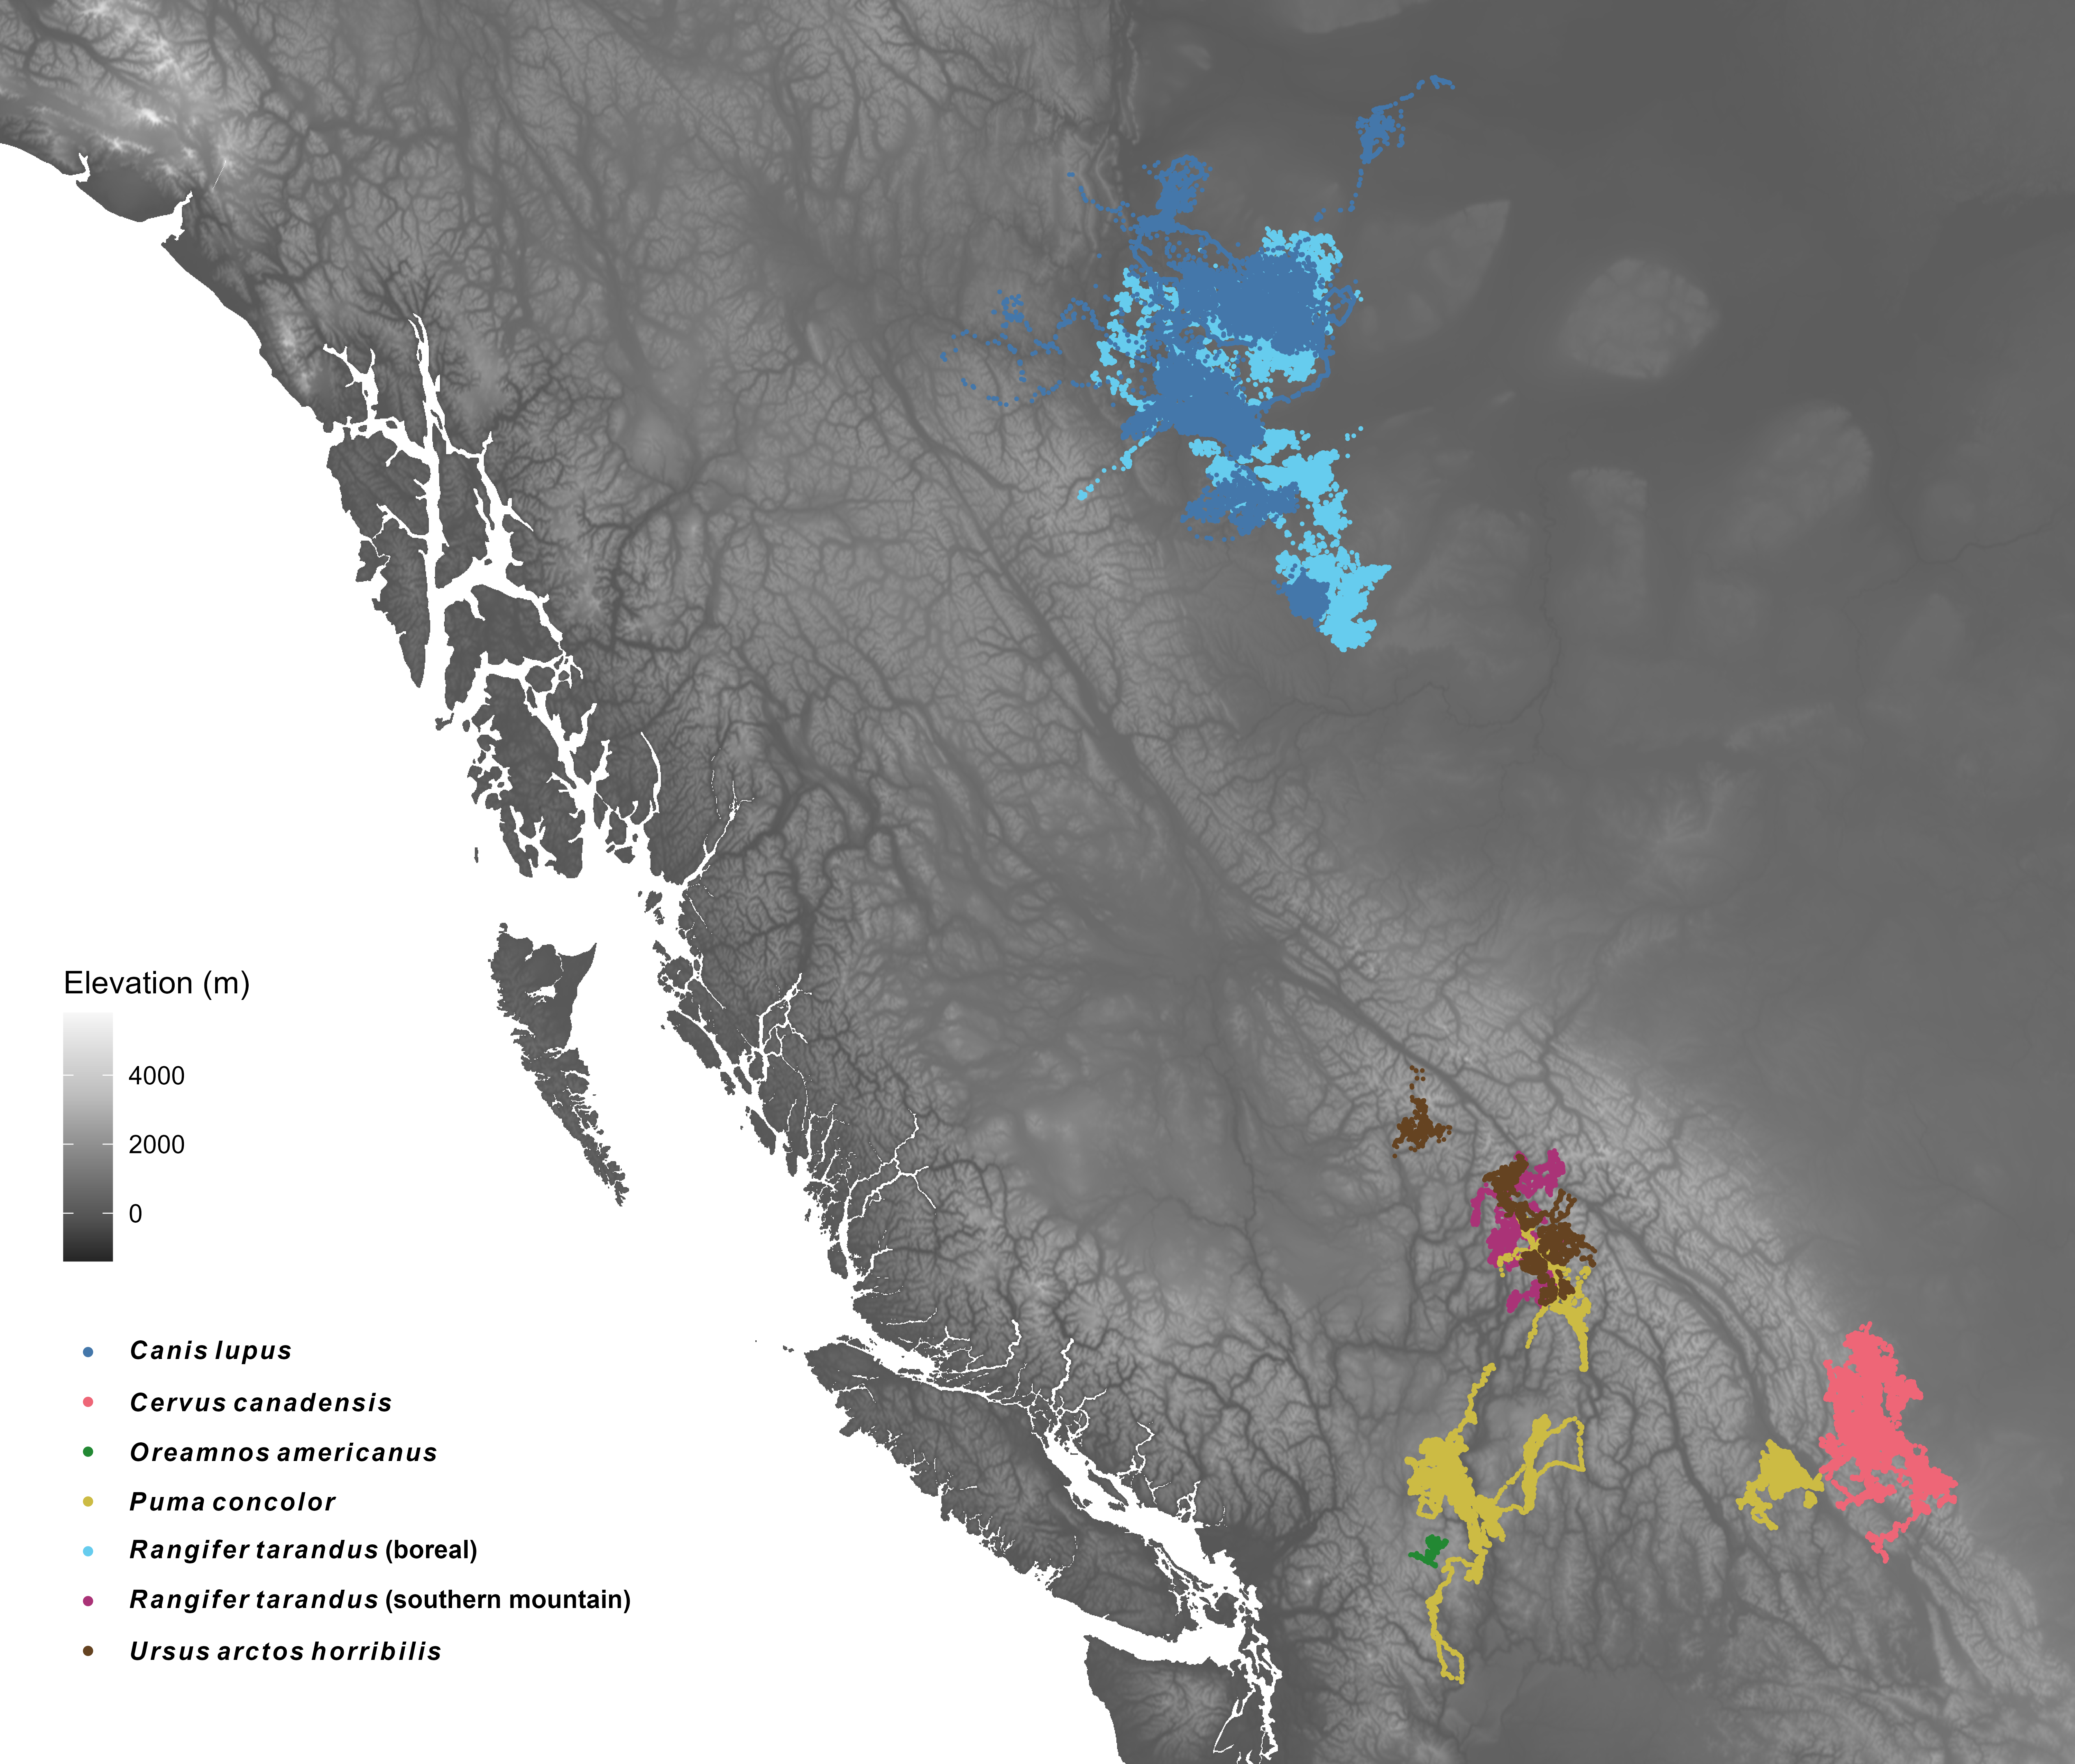
\includegraphics[width=\linewidth]{../figures/tels-map-dem} 

}

\caption{GPS telemetry data for the six species in this study (dots) over a digital elevation model for the study area. The inset in the bottom left shows the telemetry data within the north american continent. Both maps use the BC Albers Equal Area Conic projection (EPSG:3005).}\label{fig:bc-map}
\end{figure}

\scriptsize

\begin{longtable}[]{@{}
  >{\raggedright\arraybackslash}p{(\linewidth - 12\tabcolsep) * \real{0.3077}}
  >{\raggedright\arraybackslash}p{(\linewidth - 12\tabcolsep) * \real{0.1209}}
  >{\raggedright\arraybackslash}p{(\linewidth - 12\tabcolsep) * \real{0.1209}}
  >{\raggedleft\arraybackslash}p{(\linewidth - 12\tabcolsep) * \real{0.0879}}
  >{\raggedleft\arraybackslash}p{(\linewidth - 12\tabcolsep) * \real{0.1209}}
  >{\raggedleft\arraybackslash}p{(\linewidth - 12\tabcolsep) * \real{0.1319}}
  >{\raggedleft\arraybackslash}p{(\linewidth - 12\tabcolsep) * \real{0.1099}}@{}}
\caption{\label{tab:data-table}Summary statistics of each species' set of GPS data, namely: the start and end of each set of GPS telemetry data, the number of GPS fixes (after data cleaning), the median sampling interval (\(\Delta t\); stratified by animal), the number of individuals (Individuals), and the number of Individuals with finite speed estimates (Has speed).}\tabularnewline
\toprule\noalign{}
\begin{minipage}[b]{\linewidth}\raggedright
Species
\end{minipage} & \begin{minipage}[b]{\linewidth}\raggedright
Start
\end{minipage} & \begin{minipage}[b]{\linewidth}\raggedright
End
\end{minipage} & \begin{minipage}[b]{\linewidth}\raggedleft
Fixes
\end{minipage} & \begin{minipage}[b]{\linewidth}\raggedleft
Δt (hours)
\end{minipage} & \begin{minipage}[b]{\linewidth}\raggedleft
Individuals
\end{minipage} & \begin{minipage}[b]{\linewidth}\raggedleft
Has speed
\end{minipage} \\
\midrule\noalign{}
\endfirsthead
\toprule\noalign{}
\begin{minipage}[b]{\linewidth}\raggedright
Species
\end{minipage} & \begin{minipage}[b]{\linewidth}\raggedright
Start
\end{minipage} & \begin{minipage}[b]{\linewidth}\raggedright
End
\end{minipage} & \begin{minipage}[b]{\linewidth}\raggedleft
Fixes
\end{minipage} & \begin{minipage}[b]{\linewidth}\raggedleft
Δt (hours)
\end{minipage} & \begin{minipage}[b]{\linewidth}\raggedleft
Individuals
\end{minipage} & \begin{minipage}[b]{\linewidth}\raggedleft
Has speed
\end{minipage} \\
\midrule\noalign{}
\endhead
\bottomrule\noalign{}
\endlastfoot
Caribou (boreal) & 2011-03-02 & 2018-01-03 & 200,561 & 13.00 & 146 & 131 \\
Caribou (southern mountain) & 1998-03-20 & 2009-06-06 & 27,921 & 6.00 & 22 & 20 \\
Cougars & 2006-02-04 & 2021-07-12 & 80,650 & 2.00 & 29 & 29 \\
Elk & 2007-01-13 & 2013-11-19 & 875,853 & 2.00 & 169 & 169 \\
Grizzly bears & 2004-09-29 & 2009-09-07 & 39,021 & 1.00 & 18 & 18 \\
Mountain goats & 2019-06-24 & 2023-10-04 & 65,452 & 6.25 & 11 & 10 \\
Wolves & 2013-01-26 & 2017-08-29 & 202,433 & 0.25 & 39 & 39 \\
\end{longtable}

\normalsize

\section{Methods}\label{methods}

\subsection{Movement and Environmental Data}\label{movement-and-environmental-data}

\noindent To estimate how temperature affected the movement and habitat selection of a community of large, Nearctic mammals, we leveraged three datasets: (1) a multi-species collection of 25 years of GPS telemetry data throughout a large spatial extent of western Canada (Fig. \ref{fig:bc-map}), (2) historical, hourly air temperature data from the ERA5 reanalyzed dataset (Hersbach \emph{et al.}, 2023), and (3) temporally static rasters of percent forest cover, elevation, and distance from water. We then forecasted each species' movement behaviour throughout the 21\textsuperscript{st} century using monthly climate change projections under four Shared Socioeconomic Pathways (SSPs\(;\) Riahi \emph{et al.}, 2017; Mahony \emph{et al.}, 2022): i) SSP 1-2.6 (Sustainability; ``Taking the Green Road''), ii) SSP 2-4.5 (``Middle of the Road''), iii) SSP 3-7.0 (Regional Rivalry; ``A Rocky Road''), and iv) SSP 5-8.5 (Fossil-fueled Development; ``Taking the Highway'').

\subsubsection{GPS telemetry data}\label{gps-telemetry-data}

\noindent Boreal caribou and wolf telemetry data (Table \ref{tab:data-table}) were acquired from a data repository of the British Columbia Oil and Gas Research and Innovation Society (BC ORGIS) that was collected as part of the boreal caribou radio-collaring program of the BC OGRIS Research and Effectiveness Monitoring Board (REMB\(;\) BC OGRIS, 2018). Southern mountain caribou data were obtained from Ford \emph{et al.} (2023), although individuals translocated from maternity pens were excluded from the analyses. Cougar data are from Darlington \emph{et al.} (2025) and Bird \emph{et al.} (2010). Elk data from Ciuti \emph{et al.} (2012) were downloaded from Movebank (Kays \emph{et al.}, 2022). Finally, grizzly bear telemetry data are from Serrouya \emph{et al.} (2011), while mountain goat data are from the work of Balyx (2022) and were provided by the British Columbia Ministry of Environment and Parks. From the full set of telemetry data, we identified and removed 2,396 outliers, which represented ca. 0.16\% of the total dataset, including collar calibration data. Full details on the outlier identification process are provided in Appendix A.

\subsubsection{Historical temperature data and climate change projections}\label{historical-temperature-data-and-climate-change-projections}

\noindent Rasters of hourly air temperature data were downloaded from the ERA5 database (Hersbach \emph{et al.}, 2023) from the European Center for Medium-range Weather Forecasting server (ECMWF; \url{www.ecmwf.int}; \url{https://cds.climate.copernicus.eu}). Proximal air temperature was estimated for each GPS location by extracting the value from the corresponding raster cell from the temporally nearest raster using the \texttt{extract()} function from the \texttt{terra} package (v. 1.7-46, Hijmans, 2023) for \texttt{R} (R Core Team, 2024).

To obtain projected average monthly temperatures from 2025 to 2100 at a 0.08\(^\circ\) spatial resolution, we used the the \texttt{climatenaR} package (v. 1.0, Burnett, 2023) for \texttt{R} and ClimateNA v. 7.4.2 (Wang \emph{et al.}, 2016; Mahony \emph{et al.}, 2022). However, the climate projections only included estimates of future monthly averages, a scale substantially coarser than that of our tracking data (Table \ref{tab:data-table}). To estimate the distribution of temperatures at an hourly scale within a month, we assumed values to be approximately normally distributed with mean temperature \(\mu_T\) and variance \(\sigma^2_T\). We estimated \(\mu_T\) using the ClimateNA projections, while we estimated \(\sigma^2_T\) by modeling the observed variance in historical weather data for western Canada from 1998 to 2023 (inclusive). For each location \(\langle x, y \rangle\) and month \(m\) of each year (e.g., the observed variance at coordinates \(\langle -119.40, 49.94 \rangle\) in April 2005), we calculated the variance in historical temperature data, for a total of \((2024 - 1998) \times 12 = 312\) observations per location. We then modeled \(\sigma^2_T\) with a Generalized Additive Model (GAM) for Location and Scale (GAMLS, Rigby \& Stasinopoulos, 2005; Stasinopoulos \& Rigby, 2007; section 7.9 in Wood, 2017) fitted with the \texttt{mgcv} package for \texttt{R} (v. 1.9-1, Wood, 2017). The linear predictor for the location (i.e., the mean) included smooth terms of: each year's estimated within-pixel monthly mean temperature (\(\hat \mu_T\)), month (\(m\)), a two-dimensional smooth of spatial coordinates \(\langle x, y \rangle\), and a tensor product interaction term of month and space to allow for seasonal terms to vary smoothly over space. The linear predictor for the scale term, which governs the mean-variance relationship (Wood, 2017), included smooth terms of the monthly mean temperature, month, and space. We did not include smooth terms of year to avoid unrealistic projections when extrapolating beyond past 2023. The complete model for the distribution of projected temperature was thus

\begin{equation}\label{eq:temp-var-model}
\begin{cases}
T \sim \text{Normal}(\mu_T, \sigma^2_T) \\
\mu_T \approx \hat \mu_T \text{ as projected by ClimateNA} \\
\sigma^2_T \sim \text{Gamma}(\mu_{\sigma^2_T}, \nu_{\sigma^2_T}) \\
\mathbb E(\sigma^2_T) = \mu_{\sigma^2_T} \\
\mathbb V(\sigma^2_T) = (\mu_{\sigma^2_T})^2 / \nu_{\sigma^2_T} \\
\log(\mu_{\sigma^2}) = \beta_{L,0} + f_{L,1}(\mu_T) + f_{L,2}(m) + f_{L,3}(x, y) + f_{L,4}(x, y, m) \\
\log(\nu_{\sigma^2}) = \beta_{S,0} + f_{S,1}(\mu_T) + f_{S,2}(m) + f_{S,3}(x, y)
\end{cases},
\end{equation}

\noindent where \(\mu_{\sigma^2_T}\) and \(\nu_{\sigma^2_T}\) indicate the location and scale parameters of the gamma distribution of \(\sigma^2_T\), and together they determine the variance of \(\sigma^2_T\), indicated as \(\mathbb V(\sigma^2_T)\). Functions \(f_{L,j}\) and \(f_{S,j}\) indicate the \(j^\text{th}\) smooth functions for the location and scale parameters, respectively. To ensure the smooth functions of month, \(f_{L,2}(m)\) and \(f_{S,2}(m)\), joined smoothly between December and January, the terms use cyclic cubic spline bases. The spatial terms used two-dimensional Duchon splines, a generalization of thin-plate regression splines (Wood, 2017). The smoothness parameters were estimated via REstricted Maximum Likelihood (REML\(;\) Wood, 2017). See the Data Availability Statement for additional information on the code used to fit the model.

We simulated hourly variation in future years by assuming hourly temperature followed a normal distribution with mean specified by the monthly \texttt{climatenaR} climate projections and variance as specified by the gamma GAMLS. For each month within each year from 2025 to 2100, we simulated hourly weather by including temperatures from the 0.1 to the 0.9 quantiles by increments of 0.1, and we weighted each quantile proportionally to the normalized Gaussian probability density for each quantile.

\subsubsection{Habitat rasters}\label{habitat-rasters}

\noindent We estimated percent forest cover and distance from water using the temporally static rasters created by Tuanmu \& Jetz (2014). We calculated total forest cover by summing the four rasters of evergreen/deciduous needle-leaf trees, evergreen broadleaf trees, deciduous broadleaf trees, and mixed/other trees (raster classes 1-4, respectively). We converted the raster of percent cover of open water (class 12) to a binary raster of pixels with water (cover \(\ge 1\% \approx 40,000 \text{m}^2\) for a \(\approx 4 \text{km}^2\) pixel) or without water (cover \(\le 1\%\)) and then calculated each pixel's distance from the nearest pixel with water using the \texttt{distance()} function from the \texttt{terra} package. We recognize that although this approach may fail to account for small or ephemeral bodies of water, it should still capture large-scale preferences for proximity to water. Finally, we obtained two digital elevation models using the \texttt{get\_elev\_raster()} function from the \texttt{elevatr} package (v. 0.99.0, Hollister \emph{et al.}, 2023). We used a raster with a zoom of 6 (a resolution of 0.009\(^\circ\)) for model fitting and one with a zoom of 3 (a resolution of 0.08\(^\circ\)) for downloading climate change projections via \texttt{climatenaR}. All final rasters and code are available on GitHub (see the Data Availability Statement).

For ease of interpretability and comparison with current conditions, we assumed resources would remain constant through to 2100, although we recognize that the spatial distribution of forest cover and open water will change throughout the 21\textsuperscript{st} century (Pochailo \emph{et al.}, 2025). We also do not account for human presence and activity, even though both have significant impacts on species' movement rates and will intensify in the coming decades (Ciuti \emph{et al.}, 2012; Johnson \emph{et al.}, 2018; Tucker \emph{et al.}, 2018; Weststrate \emph{et al.}, 2024).

\subsection{Estimating mammals' instantaneous speeds}\label{estimating-mammals-instantaneous-speeds}

\noindent We modeled each animal's movement using continuous-time movement models (Fleming \emph{et al.}, 2014) via the \texttt{ctmm} package (v. 1.2.0, Fleming \& Calabrese, 2023) for \texttt{R}. We then estimated each mammal's instantaneous speed at each observed location by applying the \texttt{ctmm::speeds()} function on all models with finite speed estimates (415 of 433\(;\) Fleming \emph{et al.}, 2014; Noonan \emph{et al.}, 2019). The remaining 18 movement models had sampling rates that were too coarse, relative to the animals' directional persistence, to reconstruct the animals' movement trajectories (Noonan \emph{et al.}, 2019; Nathan \emph{et al.}, 2022; DeNicola \emph{et al.}, 2025). The models were for one mountain goat, 15 boreal caribou, and two southern mountain caribou (Table \ref{tab:data-table}). Our use of continuous-time estimates of instantaneous speed mitigated the effects of varying sampling intervals across individuals (Noonan \emph{et al.}, 2019; Nathan \emph{et al.}, 2022).

Since \(\texttt{ctmm}\text{'s}\) movement models assume a single moving state with stochastic but non-zero speed (Calabrese \emph{et al.}, 2016; Noonan \emph{et al.}, 2019), we corrected data-informed speeds so that the minimum instantaneous speed could be 0. We performed this correction by subtracting each model's mean speed while assuming speeds were \(\chi^2\)-distributed. To avoid artifacts due to excessively small, non-zero speeds, we determined whether an animal was moving or not using a \(k\)-means algorithm with 2 clusters for each species' distribution of detrended speeds. When the algorithm clearly failed to discriminate between states, we estimated the split point using the inflection points in histograms of the detrended speeds (Fig. B1).

\subsection{Estimating the effects of temperature on mammals' movement behaviour}\label{estimating-the-effects-of-temperature-on-mammals-movement-behaviour}

\noindent Ambient temperature is only one of the many drivers of mammalian movement behaviour (Fig. \ref{fig:dags}). Many species alter their movement rates (e.g., movement frequency and speed) daily or seasonally in response in factors such as solar time, photoperiod, forage availability, reproductive cycles, and predator avoidance. Similarly, ambient temperature also fluctuates throughout the day and across seasons. Therefore, estimating the effects of temperature on movement rates requires accounting for how mammals' response to temperature changes with time of day and day of year (Fig. \ref{fig:dags}A\(;\) Webb \emph{et al.}, 2010; Buderman \emph{et al.}, 2018; Guiden \& Orrock, 2020; Leclerc \emph{et al.}, 2021; Xu \emph{et al.}, 2021). Similarly, mammals' selection strength for resources depends on ambient temperature, since higher temperatures can promote a selection for refuge from heat (e.g., thicker forest cover, higher elevation, proximity to water\(;\) Attias \emph{et al.}, 2018; Giroux \emph{et al.}, 2023; Noonan \emph{et al.}, 2026).

To assess the importance of including temperature as an explicit covariate (as opposed to including its effects with time of day and day of year), we fit models with and without smooth effects of temperature and compared the fits of the two sets of models via analyses of deviance (a form of generalized likelihood ratio tests) following Wood (2017) (also see Appendix B).

\begin{figure}

{\centering \includegraphics[width=\linewidth]{manuscript_files/figure-latex/dags-1} 

}

\caption{Directed Acyclical Graphs (DAGs) assumed for inferring the causal effects of temperature (red) on each species' movement behaviour. (A) Ambient temperature affects mammals' movement rates (i.e. probability of moving, speed when moving, and their product: hourly distance traveled). The effects of temperature on mammals' movement rates depend on circadian rhythm and phenology, since animals may respond to temperatures differently at different times of day and or days of year. Additionally, temperature varies with time of day and day of year. Finally, circadian rhythm changes with seasonal phenology due to changes in photoperiod (e.g., the time of twilight changes throughout the year, affecting crepuscular activity). (B) Similarly, habitat selection depends on the availability and selection of habitat variables (forest cover, elevation, and distance from water), but the selection strengh for each variable is conditional on temperature. For example, an animal may select for more densely-forested areas at extreme temperatures. The resource selection functions for (B) also included marginal smooths of temperature to account for sampling biases across seasons.}\label{fig:dags}
\end{figure}

\subsubsection{Effects of temperature on movement rates}\label{effects-of-temperature-on-movement-rates}

\noindent We estimated the effects of temperature on mammals' instantaneous movement state (moving or not) and speed when moving using two Hierarchical Generalized Additive Models (HGAMs\(;\) Pedersen \emph{et al.}, 2019 and Appendix B) with the \texttt{mgcv} package for \texttt{R}. The first HGAM estimated the probability that an animal was moving, \(P(M)\), with a binomial family of distributions and logit link function. The second HGAM estimated an animal's speed when moving with a gamma family of distributions and log link function. We fit the models with fast Restricted Maximum Likelihood (\texttt{\textquotesingle{}fREML\textquotesingle{}}) and discretized covariates (\texttt{discrete\ =\ TRUE}) to optimize computational efficiency with no appreciable losses to model performance (Appendix B\(;\) Wood \emph{et al.}, 2015, 2017; Li \& Wood, 2020). Together, the binomial HGAM and the gamma HGAM inform us on an animal's long-term average speed, since it is the product of the probability of moving and its average speed when moving.

The HGAMs (equations \eqref{eq:p-moving-model} and \eqref{eq:speed-model}) included fixed-effect intercepts for each species (\(\beta_\texttt s\)), random intercepts for each animal (\(Z_\texttt{a}\)), and species-level \texttt{by} smooths that allowed independent smoothness parameters for each species (Pedersen \emph{et al.}, 2019). The \texttt{by} smooths accounted for trends in time of day (in Pacific Daylight Time; \texttt{tod\_pdt}), day of year (\texttt{doy}), and temperature (\texttt{temp\_c}). To account for the cyclicity of time of day and day of year, the smooth terms used cyclic cubic splines (Wood, 2017). The models also had three tensor product interaction terms \texttt{by} each species: (1) day of year and time of day, (2) temperature and time of day, and (3) temperature and day of year. These three terms accounted for smooth changes in: (1) daily behaviour across day of year, (2) the response to temperature over time of day (e.g., changes in nocturnality), and (3) the response to temperature over day of year (e.g., the timing of molting, migration, and hibernation). Finally, two smooth terms of log-transformed sampling interval (\texttt{dt}; hours) corrected for biases in speed estimates arising from irregular GPS sampling intervals, since longer intervals result in lower speed estimates (Nathan \emph{et al.}, 2022; DeNicola \emph{et al.}, 2025). A global smooth term of \(\log(\texttt{dt})\) accounted for the overall effect of sampling interval, while a factor-smooth interaction term (\texttt{bs\ =\ \textquotesingle{}fs\textquotesingle{}}) of \(\log(\texttt{dt})\) and species accounted for species-level deviations from the global term while assuming a common smoothness parameter across species (Pedersen \emph{et al.}, 2019). Formally, the model for movement state \(M\), with \(M = 0\) indicating no movement and \(M = 1\) indicating movement, was

\begin{equation}\label{eq:p-moving-model}
\begin{cases}
M \sim \text{Bin}(p) \\
\mathbb E(M) = p \\
\mathbb V(M) = p (1-p) \\
\begin{aligned}
\text{logit}(p) = & \beta_\texttt{s} + Z_\texttt{a} + f_{1,\texttt{s}}(\texttt{tod\_pdt}) + f_{2,\texttt s}(\texttt{doy}) + f_{3,\texttt s}(\texttt{temp\_c}) + \\
& f_{4,\texttt s}(\texttt{doy}, \texttt{tod\_pdt}) + f_{5, \texttt s}(\texttt{temp\_c}, \texttt{tod\_pdt}) + f_{6, \texttt s}(\texttt{temp\_c}, \texttt{doy}) + \\
& f_7(\log(\texttt{dt})) + f_{8,\texttt s}(\log(\texttt{dt}))
\end{aligned}
\end{cases},
\end{equation}

\noindent while the model for movement speed when moving (i.e., \(M = 1\), indicated with \(S\)) was

\begin{equation}\label{eq:speed-model}
\begin{cases}
S \sim \text{Gamma}(\mu_S, \nu_S) \\
\mathbb E(S) = \mu_S \\
\mathbb V(S) = \mu_S^2 / \nu_S \\
\begin{aligned}
\text{log}(\mu_S) = & \beta_\texttt{s} + Z_\texttt{a} + f_{1,\texttt{s}}(\texttt{tod\_pdt}) + f_{2,\texttt s}(\texttt{doy}) + f_{3,\texttt s}(\texttt{temp\_c}) + \\
& f_{4,\texttt s}(\texttt{doy}, \texttt{tod\_pdt}) + f_{5, \texttt s}(\texttt{temp\_c}, \texttt{tod\_pdt}) + f_{6, \texttt s}(\texttt{temp\_c}, \texttt{doy}) + \\
& f_7(\log(\texttt{dt})) + f_{8,\texttt s}(\log(\texttt{dt}))
\end{aligned}
\end{cases}.
\end{equation}

\noindent In both models, \(\beta_\texttt{s}\) indicates a fixed intercept for species \texttt{s}, \(Z_\texttt a\) indicates a Gaussian random effect for animal \texttt{a} (of species \texttt{s}), \(f_{j,\texttt{s}}\) indicates the \(j^{\text{th}}\) smooth function for species \texttt{s}, and functions with two variables indicate tensor product interaction terms. Sampling interval affected estimates of probability as well of as speed when moving (Fig. B8). All species' estimated probability of moving and speed when moving decreased with sampling intervals above 1 hour, except for cougars' speed, although the estimated trends were highly uncertain (Fig. B8). Consequently, we present all results while predicting specifically for one-hour sampling intervals. The model code used to fit the models is available in Appendix B.

\subsubsection{Effects of temperature on habitat selection}\label{effects-of-temperature-on-habitat-selection}

\noindent We estimated the effects of temperature on each species' selection for percent forest cover (\texttt{forest\_perc}), elevation (\texttt{elevation\_m}, in meters), and distance from water (\texttt{dist\_water\_m}, in meters) by fitting a Hierarchical Resource Selection Function (HRSF) for each species (McCabe \emph{et al.}, 2021). These three variables were selected to balance generality across a taxonomically and ecologically diverse community while also ensuring ecological relevance to temperature-dependent habitat selection. Forest cover provides shade and reduces ambient temperature experienced by individuals, and many species are documented to select for denser canopy cover as temperatures rise (Attias \emph{et al.}, 2018; Giroux \emph{et al.}, 2023; Noonan \emph{et al.}, 2026). Elevational shifts in habitat use are a well-known response to warming temperatures, and have been documented across a wide range of taxa (White \& Gregovich, 2017; McCain, 2019; Carbeck \emph{et al.}, 2022; Lamb \emph{et al.}, 2025). Proximity to water provides direct thermoregulatory benefits through wallowing and drinking, reduces heat stress, and is associated with riparian vegetation that can provide additional thermal refuge (Dobrowski, 2011; McLaughlin \emph{et al.}, 2017; Fuller \emph{et al.}, 2021; Verzuh \emph{et al.}, 2023; Zhang \emph{et al.}, 2023b). Collectively, these variables represent three of the primary means by which large mammals in temperate, boreal systems can respond to thermal stress via changes in habitat use (Stralberg \emph{et al.}, 2020), while remaining estimable from globally available, temporally static rasters that facilitate straightforward climate change projections.

We fit each HRSF using an HGAM with a Poisson family of distributions and log link function (Appendix B\(;\) Aarts \emph{et al.}, 2008). After removing non-resident individuals (Table B1), we accounted for the spatiotemporal autocorrelation in the telemetry locations by weighting each point based on the telemetry's Autocorrelated Kernel Density Estimate (Alston \emph{et al.}, 2022) to produce estimates of second-order habitat selection (\emph{sensu} Johnson, 1980). Quadrature points were used to approximate the likelihood function of a Poisson point process through numerical integration (Baddeley \emph{et al.}, 2015) and were determined using the raster cells in each animal's 99.9\% AKDE percentile. The number of quadrature locations greatly outnumbered the number of observed locations (Fig. B12), especially after accounting for the AKDE weights (Fig. B13), which is essential for ensuring parameter convergence (Fithian \& Hastie, 2013).

Each species' model had the same structure:

\begin{equation}\label{eq:hrsf}
\begin{cases}
O \sim \text{Pois}(\lambda) \\
\mathbb E(O) = \mathbb V(O) = \lambda \\
\begin{aligned}
\text{log}(\lambda) = & \beta_0 + f_{1}(\texttt{forest\_perc}) + f_{2}(\texttt{elevation\_m}) + f_{3}(\texttt{dist\_water\_m}) + \\
& Z_\texttt a + f_{4, \texttt{a}}(\texttt{forest\_perc}) + f_{5, \texttt{a}}(\texttt{elevation\_m}) + f_{6, \texttt{a}}(\texttt{dist\_water\_m}) + \\
& f_{7}(\texttt{forest\_perc}, \texttt{temp\_c}) + f_{8}(\texttt{elevation\_m}, \texttt{temp\_c}) + \\
& f_{9}(\texttt{dist\_water\_m}, \texttt{temp\_c}) + f_{10}(\texttt{temp\_c}) + f_{11,\texttt a}(\texttt{temp\_c}))
\end{aligned}
\end{cases},
\end{equation}

\noindent where \(O\) indicates whether an animal was observed (\(O = 1\)) or not (\(O = 0\)), and the species-level indices are omitted for readability, but each term in the model can be assumed to be species-specific. Smooth effects of percent forest cover (\texttt{forest\_perc}), elevation (\texttt{elevation\_m}, in meters), and distance to water (\texttt{dist\_water\_m}, in meters) accounted for the species-level selection strength for each resource. A Gaussian random effect for each individual animal (\(Z_\texttt a\)) corrected for uneven sampling across individuals, while factor-smooth interaction terms for each animal (\(f_{j,\texttt a}\)) accounted for animal-level resource selection (i.e., individual-level deviations from the species-level estimate\(;\) Jeltsch \emph{et al.}, 2025). Tensor product interaction terms of the three resources and temperature (\texttt{temp\_c}) estimated the smooth change in resource selection at different temperatures. Finally, marginal smooth terms of temperature and factor-smooth interaction terms of temperature and animal accounted for species- and individual-level sampling biases at different temperatures (e.g., sampling more during warm periods).

\section{Results}\label{results}

\noindent Across species, approximately 10\% of GPS fixes had absolute temperatures above \(20^\circ\)C. Of the fixes with finite speed estimates, 2.6\% had temperatures lower than \(-20^\circ\)C, while 6.5\% had temperatures above \(20^\circ\)C, but temperature ranges differed across species (Table \ref{tab:hgam-summary}, Fig. B2). At \(0^\circ\)C, species differed in estimated mean probabilities of moving (\(\hat P(M = 1)\); range: 0.05 -- 0.31), mean speed when moving (\(\hat {\mathbb E}(S|M=1)\); range: 0.42 -- 2.67 km/h), and mean overall speed (i.e., \(\hat P(M) \times \hat {\mathbb E}(S|M=1)\), range: 0.04 -- 0.61 km/h; Table \ref{tab:hgam-summary}). Grizzly bears had the lowest movement frequency (\(\hat P(M) \approx 0.05\)), while wolves and cougars moved most often (\(\hat P(M) \ge 0.22\)). Mountain goats and southern mountain caribou moved the slowest (\(\hat{\mathbb E}(S|M = 1) \approx 0.43\) km/h), while wolves had the highest mean speed when moving (\(\hat{\mathbb E}(S|M = 1) \approx 2.67\) km/h). Consequently, at \(0^\circ\)C, wolves traveled an average of \(0.22 \times 2.67~\text{km/h} \approx 0.6\) km/h; 2.5 to 16.7 times faster than other species.

\scriptsize

\begin{longtable}[]{@{}
  >{\centering\arraybackslash}p{(\linewidth - 12\tabcolsep) * \real{0.1361}}
  >{\centering\arraybackslash}p{(\linewidth - 12\tabcolsep) * \real{0.0651}}
  >{\centering\arraybackslash}p{(\linewidth - 12\tabcolsep) * \real{0.1479}}
  >{\centering\arraybackslash}p{(\linewidth - 12\tabcolsep) * \real{0.1479}}
  >{\centering\arraybackslash}p{(\linewidth - 12\tabcolsep) * \real{0.1361}}
  >{\centering\arraybackslash}p{(\linewidth - 12\tabcolsep) * \real{0.1953}}
  >{\centering\arraybackslash}p{(\linewidth - 12\tabcolsep) * \real{0.1716}}@{}}
\caption{\label{tab:hgam-summary}Summary statistics for each species' GPS fixes with finite speed estimates, namely: the number fixes after data cleaning (\(n\)), the percentage of fixes with temperature (\(T\)) below \(-20^\circ\)C and above \(20^\circ\)C, the estimated mean probability of moving (\(\hat P(M=1)\)), the mean speed when moving (\(\hat{\mathbb E}(S|M=1)\); km/h), and the mean hourly distance travelled (\(\hat P(M=1) \times \hat{\mathbb E}(S|M=1) = \hat{\mathbb E}(D)\); km/h), for a sampling interval of 1 hour and a temperature of \(T = 0^\circ\)C.}\tabularnewline
\toprule\noalign{}
\begin{minipage}[b]{\linewidth}\centering
Species
\end{minipage} & \begin{minipage}[b]{\linewidth}\centering
\(n\)
\end{minipage} & \begin{minipage}[b]{\linewidth}\centering
T\textless-20\textdegree{}C (\%)
\end{minipage} & \begin{minipage}[b]{\linewidth}\centering
T\textgreater+20\textdegree{}C (\%)
\end{minipage} & \begin{minipage}[b]{\linewidth}\centering
\(\hat{P}(M=1\vert T)\)
\end{minipage} & \begin{minipage}[b]{\linewidth}\centering
\(\hat{\mathbb E}(S\vert M=1,T)\)
\end{minipage} & \begin{minipage}[b]{\linewidth}\centering
\(\hat{\mathbb E}(D\vert T)\)
\end{minipage} \\
\midrule\noalign{}
\endfirsthead
\toprule\noalign{}
\begin{minipage}[b]{\linewidth}\centering
Species
\end{minipage} & \begin{minipage}[b]{\linewidth}\centering
\(n\)
\end{minipage} & \begin{minipage}[b]{\linewidth}\centering
T\textless-20\textdegree{}C (\%)
\end{minipage} & \begin{minipage}[b]{\linewidth}\centering
T\textgreater+20\textdegree{}C (\%)
\end{minipage} & \begin{minipage}[b]{\linewidth}\centering
\(\hat{P}(M=1\vert T)\)
\end{minipage} & \begin{minipage}[b]{\linewidth}\centering
\(\hat{\mathbb E}(S\vert M=1,T)\)
\end{minipage} & \begin{minipage}[b]{\linewidth}\centering
\(\hat{\mathbb E}(D\vert T)\)
\end{minipage} \\
\midrule\noalign{}
\endhead
\bottomrule\noalign{}
\endlastfoot
Caribou (boreal) & 187,679 & 6.8 & 7.9 & 0.18 & 0.73 & 0.13 \\
Caribou (s. mountain) & 26,518 & 1.3 & 3.4 & 0.11 & 0.42 & 0.05 \\
Cougars & 80,621 & 0.7 & 6.9 & 0.31 & 0.76 & 0.24 \\
Elk & 875,682 & 2.4 & 4.9 & 0.17 & 0.57 & 0.10 \\
Grizzly bears & 39,001 & 0.0 & 8.4 & 0.05 & 0.72 & 0.04 \\
Mountain goats & 65,219 & 0.7 & 2.8 & 0.13 & 0.42 & 0.06 \\
Wolves & 202,386 & 1.7 & 13.0 & 0.22 & 2.67 & 0.60 \\
Total & 1,477,106 & 2.6 & 6.5 & & & \\
\end{longtable}

\normalsize

Across all species, Relative Selection Strength (RSS) was weakest for forest cover and strongest for elevation. At temperatures near 0\(^\circ\)C, boreal caribou selected for forest cover between 50\% and 75\%, elevations near 500 m above sea level, and distances from water \textless{} 10 km, while southern mountain caribou selected for dense forest cover, elevations near 2,000 m, and distances from water \(\lessapprox\) 5 km. Cougars selected for dense forest cover (\textgreater{} 75\%), an elevation of \textasciitilde{} 1,000 m, and distances from water \textless{} 7.5 km. Elk selected for intermediate forest cover (\(\approx\) 50\%), elevations between 1,000 and 2,000 m, and distances from water of 10-15 km. Grizzly bears selected for relatively sparse forest cover (25-50\%), elevation between 1,000 and 2,000 m, and distances from water \textless{} 3 km. Mountain goats selected for sparse forest cover (\textless{} 25\%), elevations near 1,800 km, and distances from water \textless{} 5 km. Finally, wolves selected for forest cover (\(\gtrapprox\) 50\%), elevations near 1,000 m, and distances from water \textless{} 5 km. There was relatively strong agreement between models with and without temperature (Figs. B3, and B14), but including temperature always resulted in better fits (all p-values \(< 2.2\times10^{-16}\); all \(\Delta\)AIC \(\le\) 342; Appendix B).

\subsection{Effects of temperature on movement rates}\label{effects-of-temperature-on-movement-rates-1}

\noindent Species' responses to temperature varied in both the direction and magnitude of change (Figs. \ref{fig:dist}, B4-B6), even after accounting for differences in daily and seasonal activity (e.g., sleeping, migration, hibernation; Figs. B4-B6). Smooth interaction terms were well-behaved and indicated clear shifts in activity over time of day and day of year for all species. The models had good in-sample prediction (Fig. B7), since they explained reasonably high proportions of the deviance (79.3\% for the gamma model and 10.7\% for the binomial model, which is relatively high for a binomial model with binary responses: McElreath, 2020). All species altered their daily and seasonal movement behaviour to changes in temperature (Fig. \ref{fig:dist}). The response was most visible in cougars. For example, in late spring they moved from evening to early morning if hourly temperatures were below \(20^\circ\)C, but if temperatures were above 20\(^\circ\)C they moved mostly between 3:00 and 6:00 AM. Throughout the year, they tended to move more when it was colder, relative to the range of temperatures at that time of year. Overall, uncertainty around the estimated effects was generally higher at extreme temperatures due to lower data availability (Figs. B4A, B5A, and B6A).

\begin{figure}

{\centering 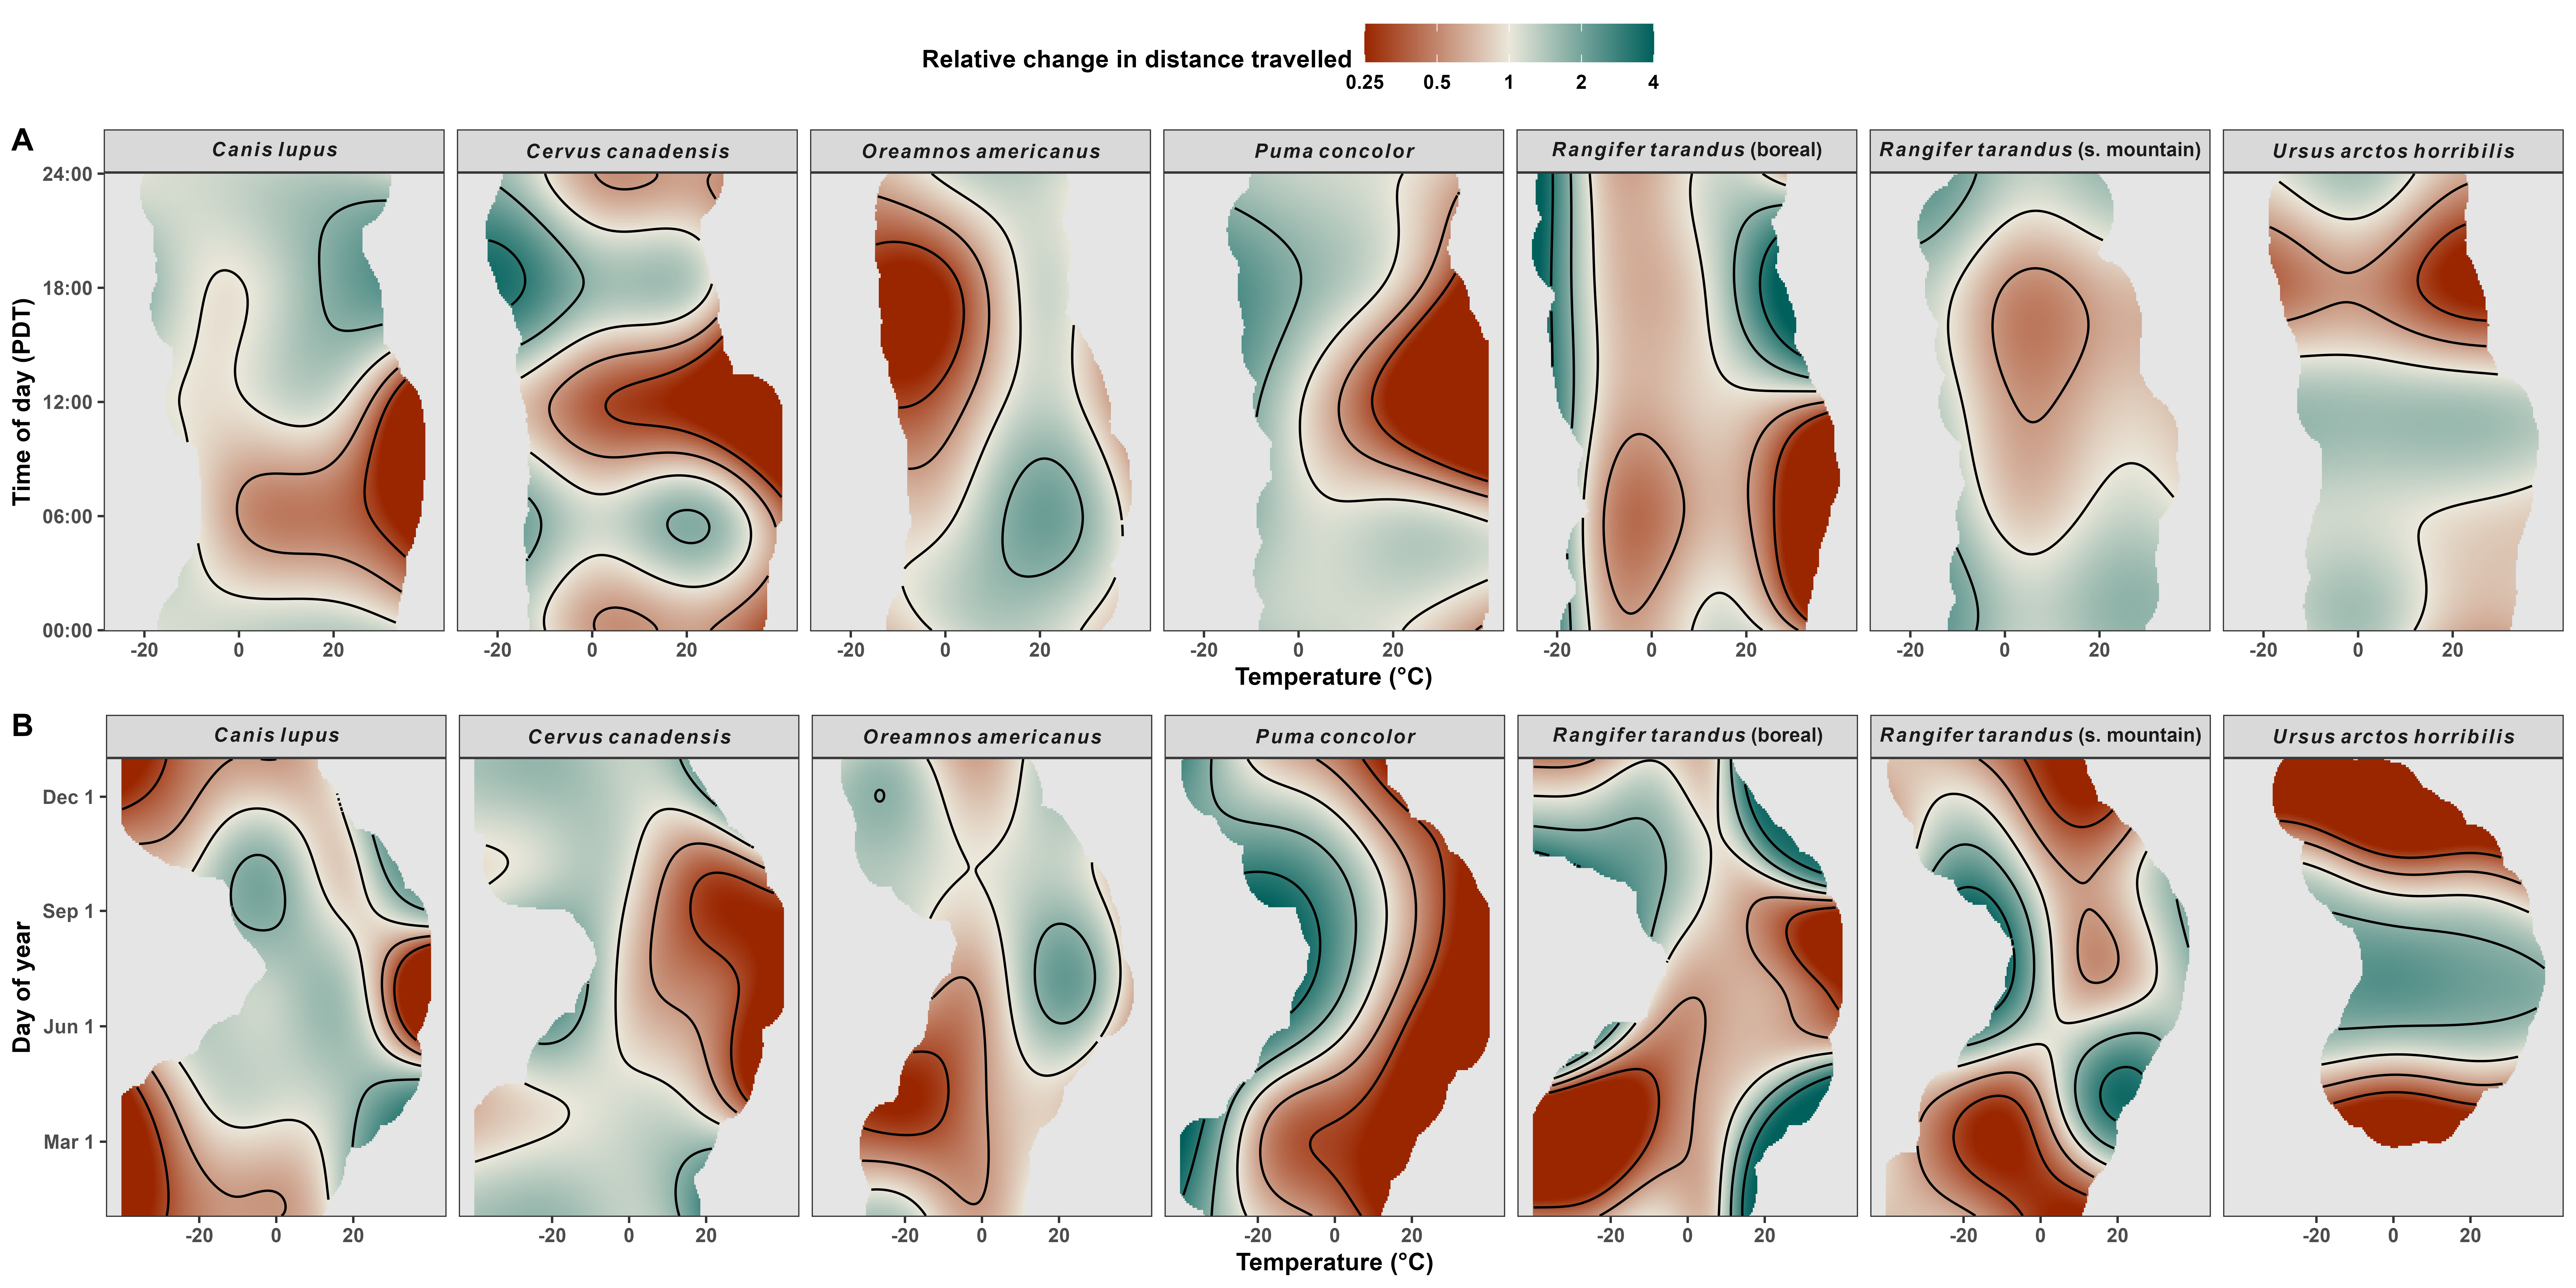
\includegraphics[width=\textwidth]{../figures/distance} 

}

\caption{\textbf{Temperature is a strong driver of how far and when mammals travel.} The fill indicates the effects of temperature on the relative change in hourly distance travelled (probability of moving times mean speed when moving) over time of day on June $1^{\text{st}}$ (\textbf{A}) and day of year at 12:00 PDT (\textbf{B}). The choices of day of year and time of day are arbitrary, but they were necessary for predicting for the tensor product interaction terms. Predictions in the surface plots extend to 10\% of the range away from each datum to avoid predicting for parameter spaces with no data (grey fill). The color bar is on the $\log_2$ scale to help visualize patterns in doubling, and values are capped to $2^{\pm 2}$ for ease of readability. Horizontal contour lines indicate that movement rates depend most on time of day and day of year (e.g., grizzly bears), while vertical lines indicate that temperature has the greatest effect, irrespective of time (e.g., mountain goats).}\label{fig:dist}
\end{figure}

\subsection{Effects of temperature on habitat selection}\label{effects-of-temperature-on-habitat-selection-1}

Species' RSS was generally strongest for elevation and weakest for forest cover, but RSS depended significantly on temperature for all species (all p-values \(< 2.2\times10^{-16}\); Fig. \ref{fig:hrsfs}). Changes in RSS with temperature were strongest for elevation and generally weakest for distance from water, but there were no common trends across all species for any of the three resources. All species except cougars exhibited clear temperature-dependent shifts in their preference for forest cover. At higher temperatures, wolves relaxed their preference for forested areas, while mountain goats relaxed their preference for open areas (cover \textless{} 50\%). As temperatures warmed, elk and boreal caribou shifted towards more forest cover closer to 50\%, while southern mountain caribou and grizzly bears selected for areas with 50\% forest cover or less. All species shifted elevationally with temperature, but species varied in the magnitude, direction, and complexity of their responses. As temperatures warmed, elk, mountain goats, and cougars moved to higher elevations, while wolves, southern mountain caribou, and grizzly bears moved to lower elevations. Cougars' selection for higher elevation strengthened substantially at temperatures \(\gtrapprox 20^\circ\)C, while mountain goats and wolves showed strong switches in preferences near \(10^\circ\)C. Wolves, elk, and southern mountain caribou moved closer to water with warmer temperature, while mountain goats, cougars, and grizzly bears moved somewhat further away from water but remained mainly within 5-10 km of water. As with movement rates, estimated RSS was generally most uncertain at extreme temperatures, for which data were scarcer (Fig. B15).

\begin{figure}

{\centering 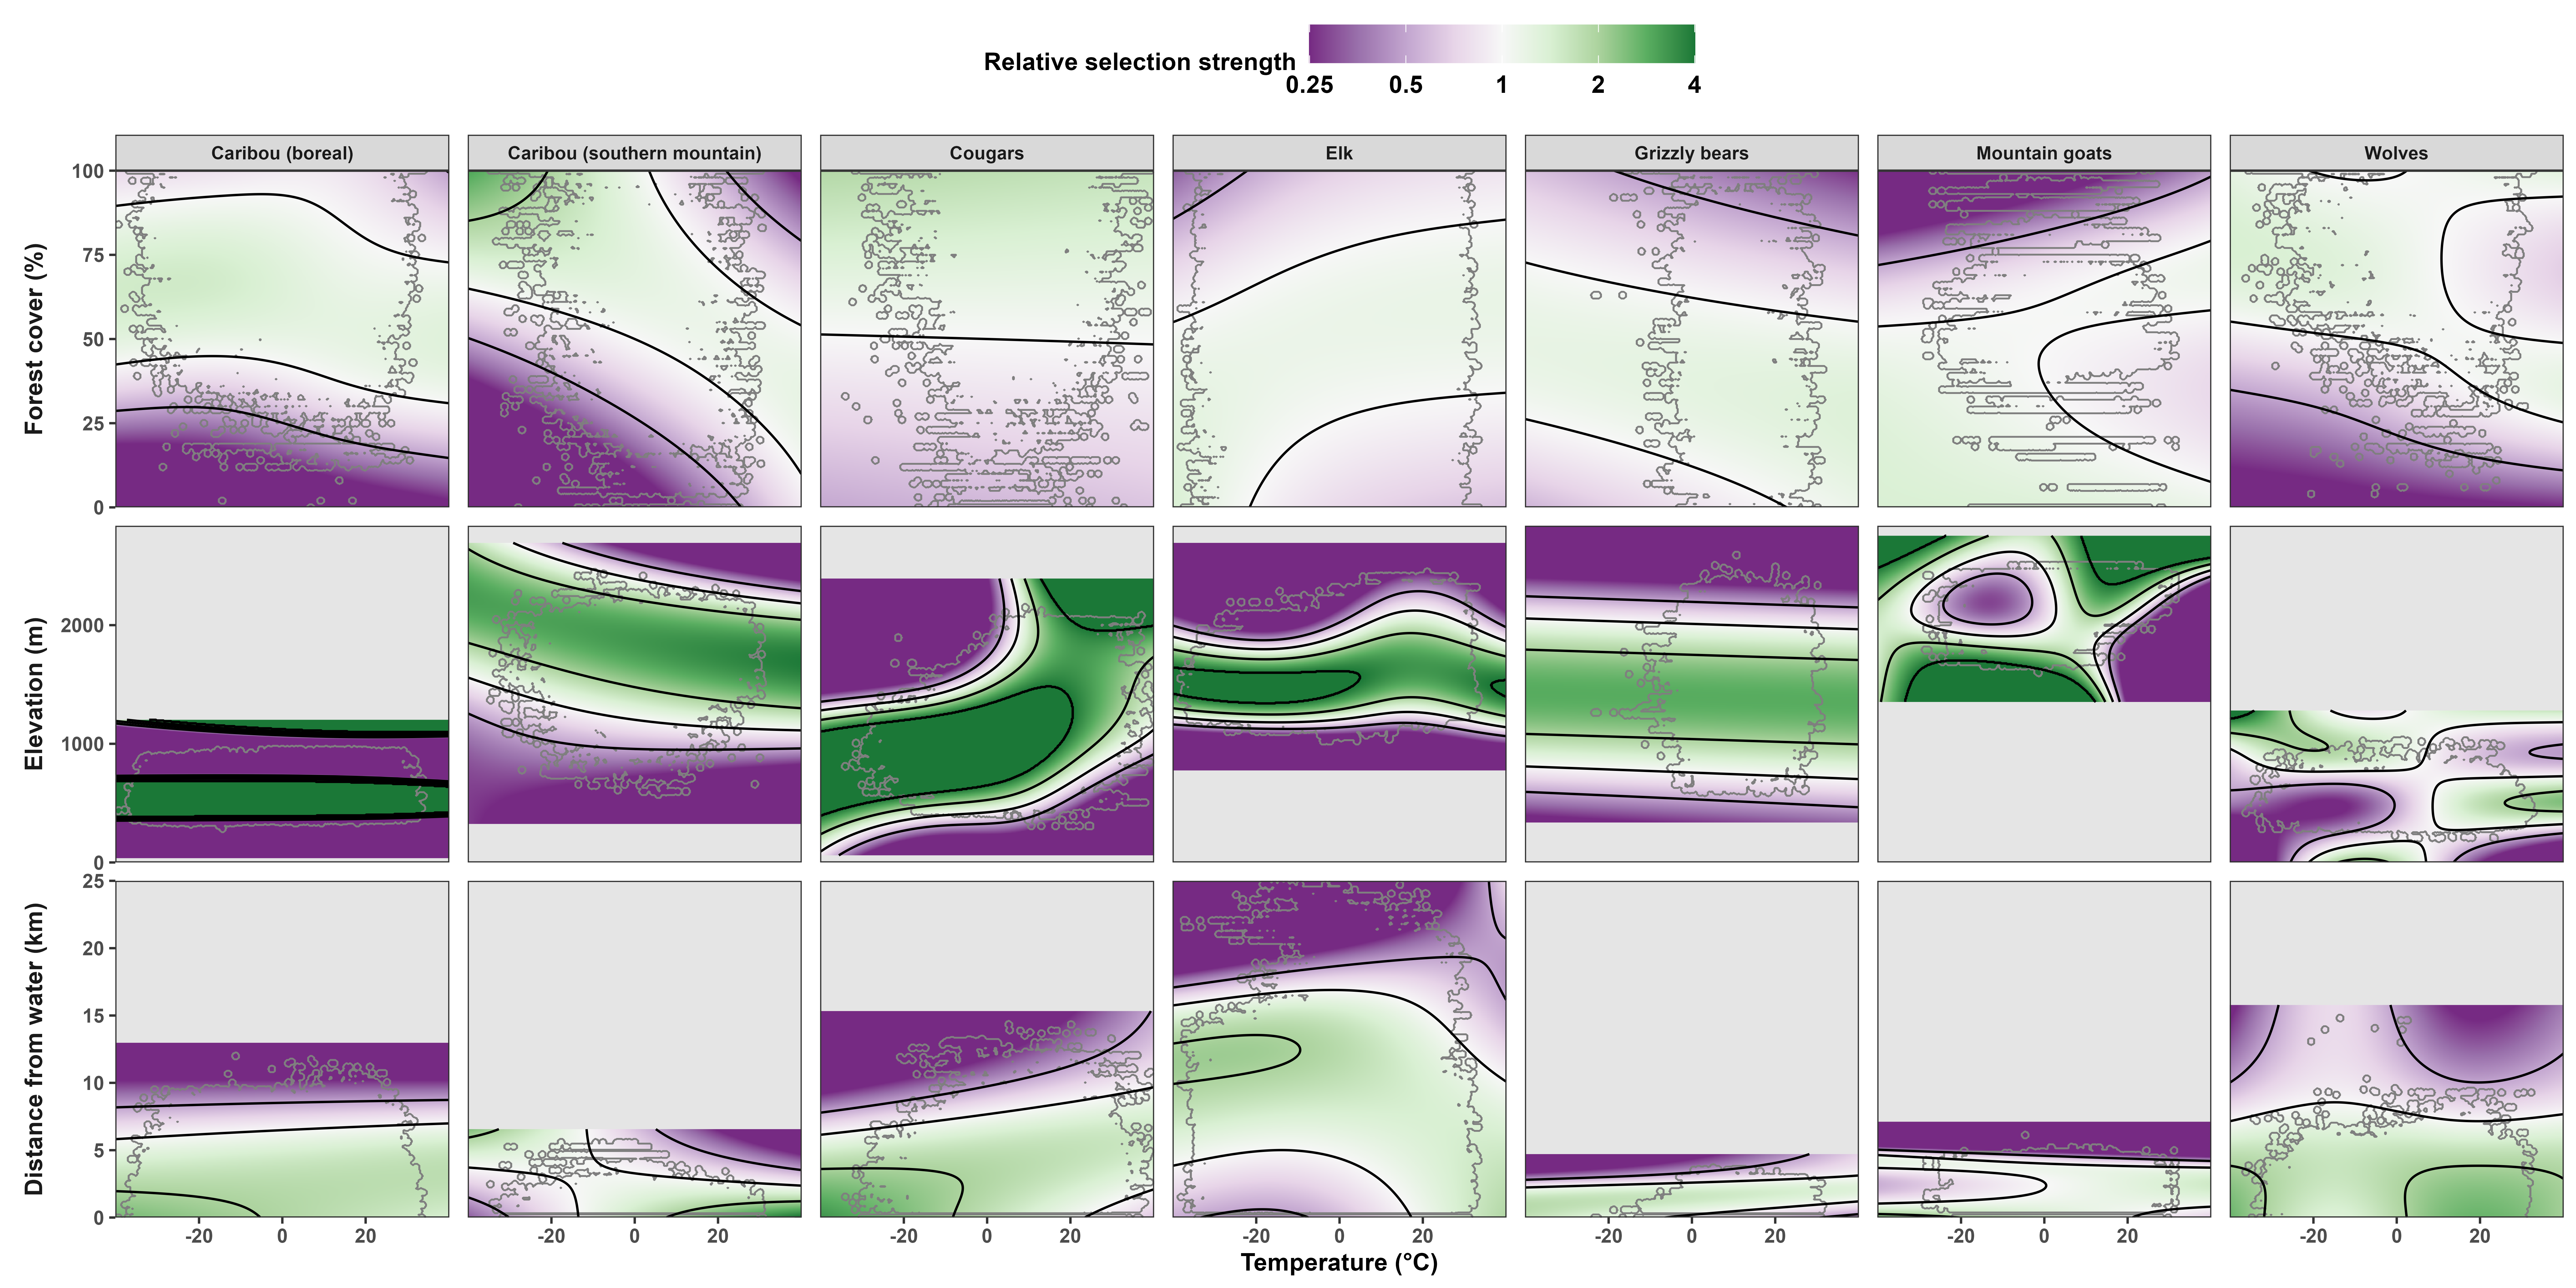
\includegraphics[width=\textwidth]{../figures/hrsf-surface-plots} 

}

\caption{\textbf{Mammals' habitat selection depends on ambient temperature.} Estimated relative selection strength (RSS) for forest cover (\%), elevation (km), and distance from water (km) as a function of temperature. The grey contours indicate the extent of each species' observed data. To mitigate the sampling bias across temperature (e.g., grizzly bears have few to no while hibernating in winter), RSS values at each temperature were divided by the average RSS value at that temperature within the respective panel. To further improve readability, each pannel's RSS values were centered by dividing by the median RSS value at $0^\circ$C and capped to between 0.25 and 4 ($2^{\pm 2}$).}\label{fig:hrsfs}
\end{figure}

Fig. \ref{fig:boreal-rss} presents a case study focusing on the predicted habitat selection for boreal caribou and wolves. We focus on these two species because their data overlap both spatially (Fig. \ref{fig:bc-map}) and temporally (Table \ref{tab:data-table}), and both species have substantial biological importance and cultural significance (Lamb \emph{et al.}, 2023), well known predator-prey dynamics (Hegel \emph{et al.}, 2010; Whittington \emph{et al.}, 2011), and complex conservation issues (Leblond \emph{et al.}, 2016; Dickie \emph{et al.}, 2017; DeMars \emph{et al.}, 2023; Labadie \emph{et al.}, 2023). Overall, both species selected for the same low-elevation area (\textless{} 500 m; Fig. \ref{fig:boreal-rss}A-B), but caribou generally avoided the river system where wolves were often found, and their selection strength varied with temperature. As wolves' habitat selection strengthened at warmer temperatures, co-occupancy at 20\(^\circ\)C was approximately four times higher than at -20\(^\circ\)C, independent of changes in the species' movement rates (Fig. \ref{fig:boreal-rss}C-D).

\begin{figure}

{\centering \includegraphics[width=\textwidth]{../figures/boreal-caribou-wolf-habitat} 

}

\caption{\textbf{Temperature affects boreal caribou's and wolves' habitat selection and, consequently, their encounter rates.} Panel (A) shows the relative selection strength (RSS) for boreal caribou and wolves, as a function of temperature. RSS values were re-centered and capped to between 0.25 and 4 ($2^{\pm 2}$) to improve readability. Panel (B) shows the rasters of the three habitat variables used in the hierarchical resource selection functions used to calculate the values in (A). Finally, panel (C) shows the (scaled) product of the RSS values in panel (B) as a proxy for the co-occupancy of the two species.}\label{fig:boreal-rss}
\end{figure}

\subsection{\texorpdfstring{Predicted changes in movement behaviour during the 21\textsuperscript{st} century}{Predicted changes in movement behaviour during the 21st century}}\label{predicted-changes-in-movement-behaviour-during-the-21st-century}

\noindent Predicted changes in movement rates with future climate change varied across species in both magnitude and direction, but worse SSPs always corresponded to greater absolute changes (Fig. \ref{fig:t-dist}). Additionally, species that were predicted to move less often did not necessarily have lower speeds when moving, and vice versa (Figs. B9 and B10). Estimated changes in average yearly distance traveled were negligible for boreal caribou and grizzly bears, although both species showed seasonal changes in seasonal movement rates. As temperatures warmed, boreal caribou were predicted to move more in winter, spring, and fall but less in summer (Fig. \ref{fig:dist}), while grizzly bears were predicted to showed a clear shift towards earlier emergence from hibernation (Fig. B4) and greater movement earlier in the year but less movement in early fall. Southern mountain caribou and mountain goats are projected to exhibit increased movement by 2100, although the estimates for southern mountain caribou varied greatly over space (Fig. \ref{fig:s-dist}). Cougars, elk, and wolves were projected to move less by 2100, with cougars showing as much as a 24\% decrease in mean yearly distance travelled.

Absolute relative changes in predicted yearly distance travelled were small under the best-case SSP (0-4\% change in 2100 relative to 2025). Under the worst-case SSP, absolute changes by 2100 (relative to 2025) ranged from \textasciitilde2\% (grizzly bears) to \textasciitilde24\% (cougars). Projected changes in 2100 varied spatially due to spatial heterogeneity in climate change projections (Fig. \ref{fig:s-dist}). Again, absolute changes were generally greatest under worse SSPs, but the direction of change at each location also varied across SSPs (most visible in cougars).

\begin{figure}

{\centering 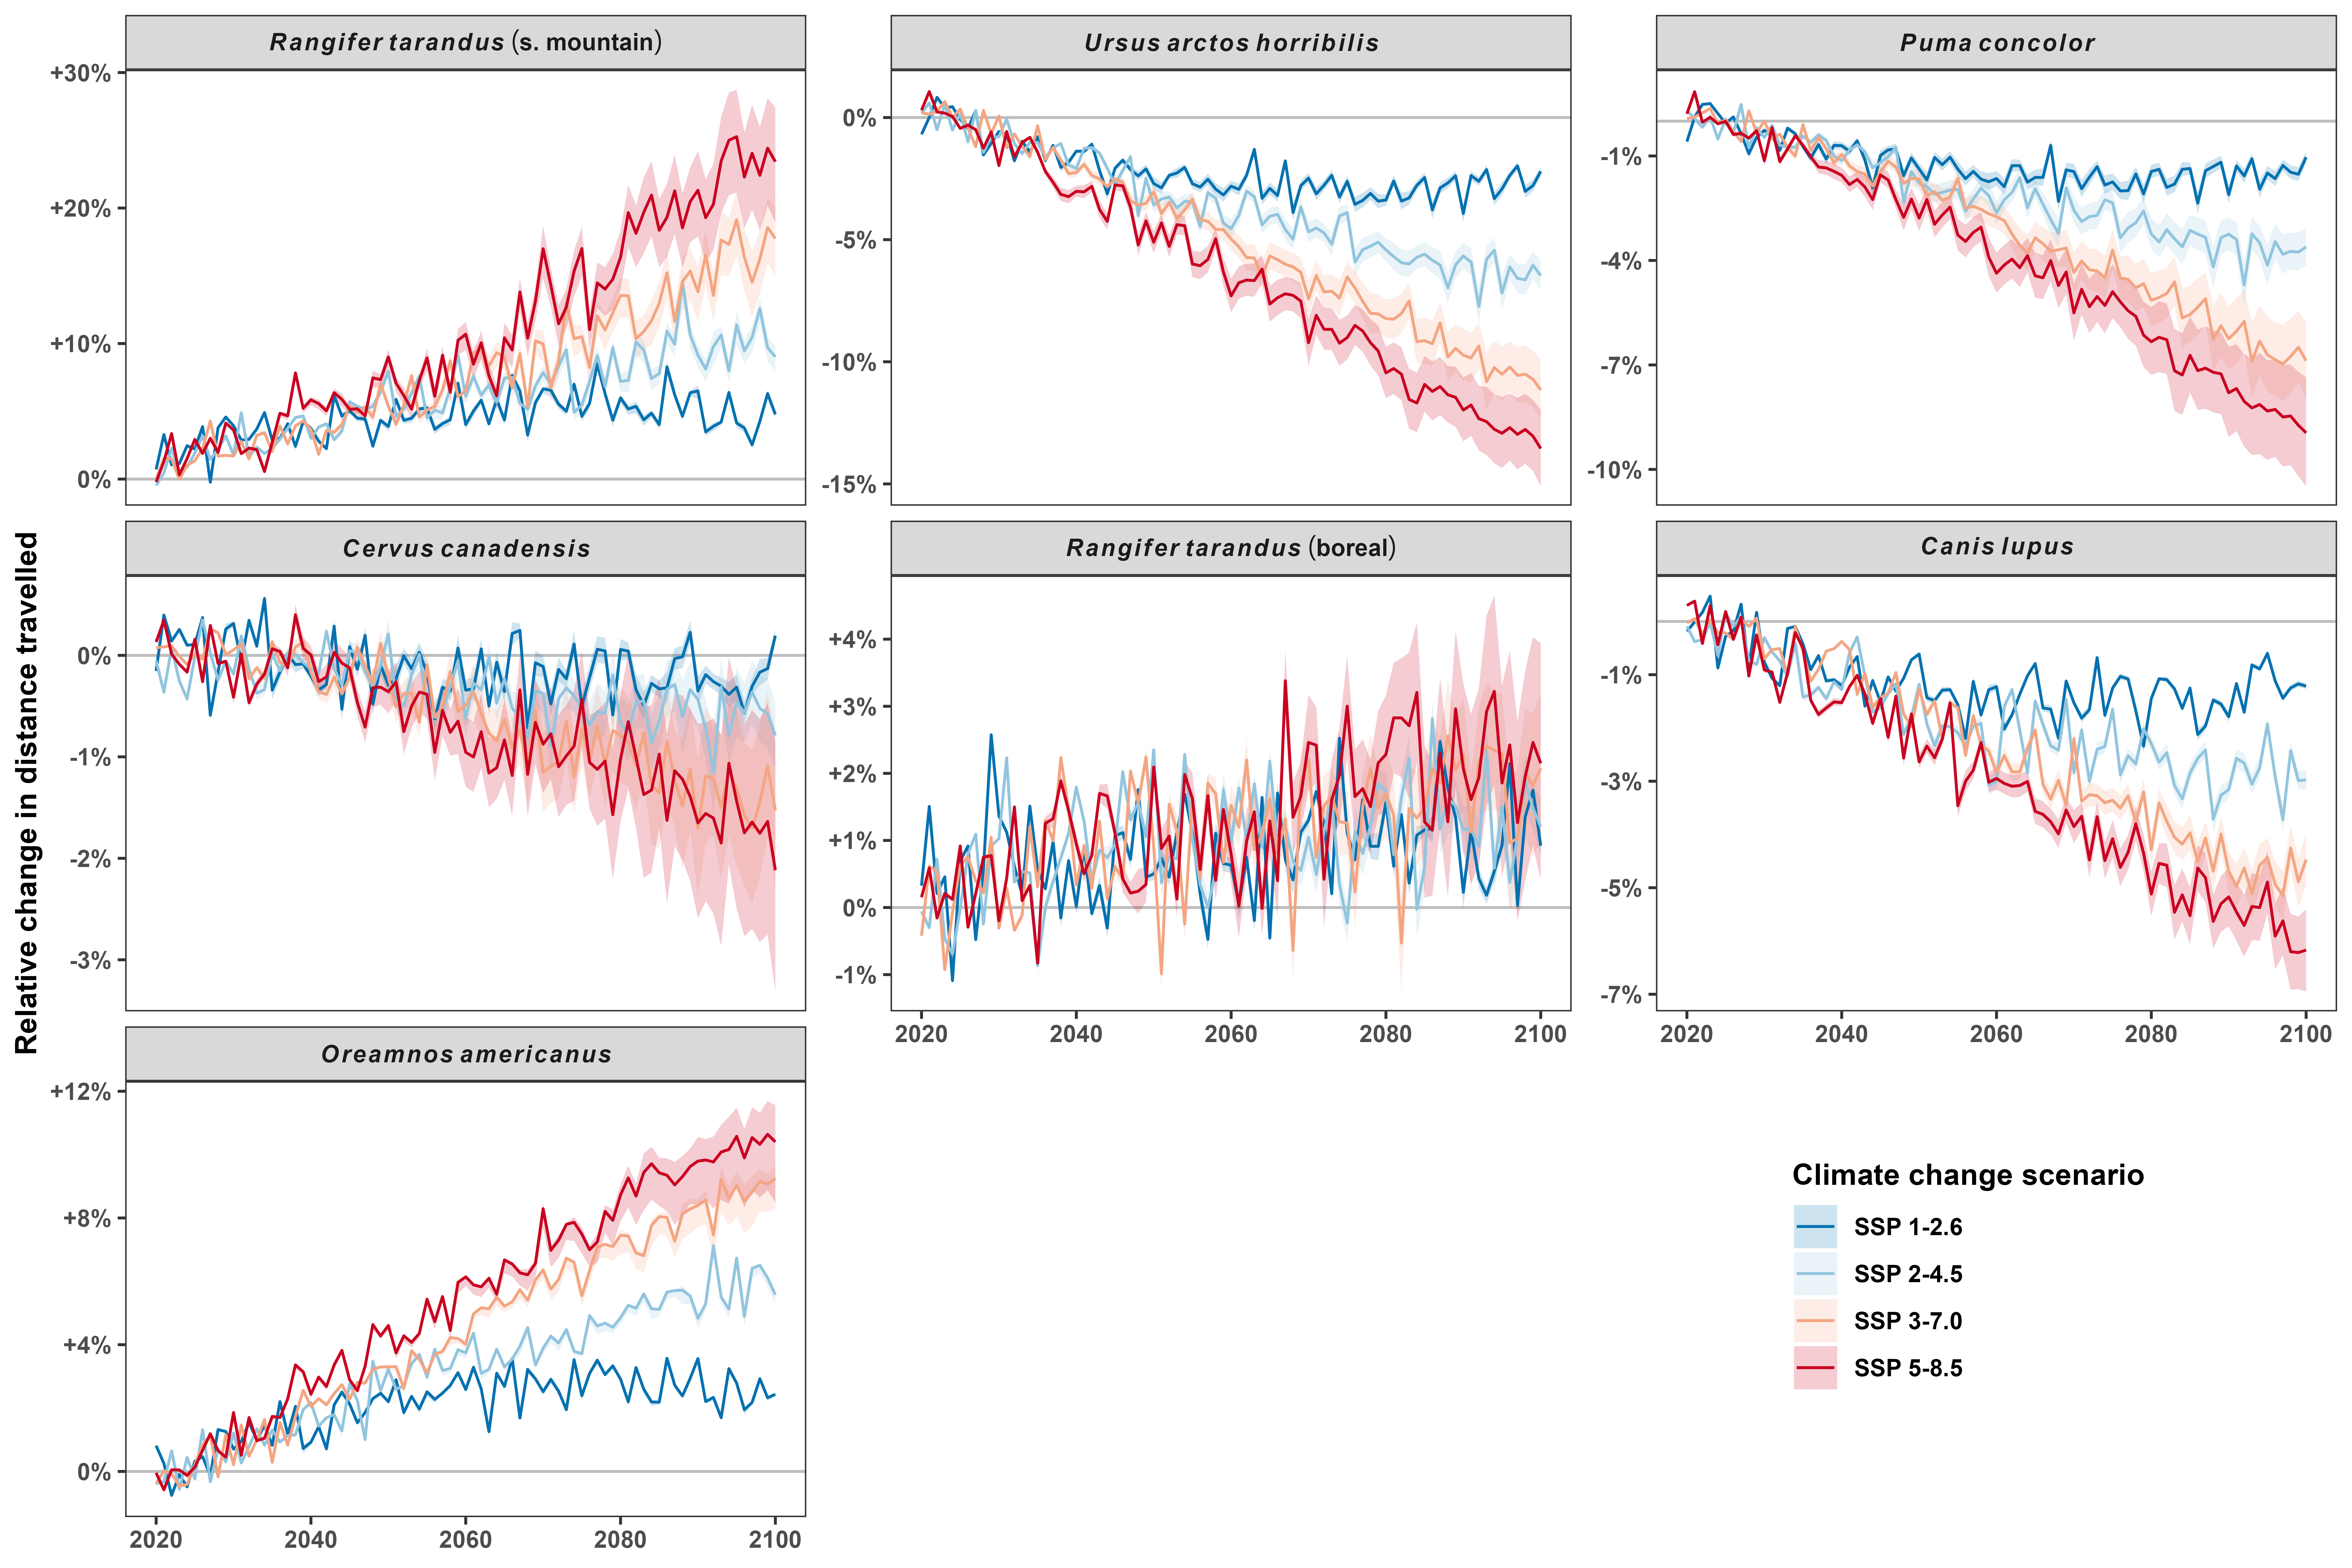
\includegraphics[width=\textwidth]{../figures/distance-travelled-local-cc-predictions} 

}

\caption{\textbf{Species are predicted to alter their movement rates differently in response to climate change, and worse climate-change scenarios will result in the greatest change.} Bold lines indicate the median change in yearly distance travelled (probability of moving times speed when moving) due to predicted changes in temperature within each species' sutdy area. Shaded areas indicate the $95^\text{th}$ and $5^\text{th}$ percentiles. Changes are relative to the mean predicted distance travelled at each location in 2025, averaged across the four Shared Socioeconomic Pathways (SSPs). Values > 1 indicate an increase, while values < 1 indicate a decrease. The projections only account for changes in movement frequency and speed, and they ignore changes in physiology or movement costs.}\label{fig:t-dist}
\end{figure}

\begin{figure}

{\centering \includegraphics[width=\textwidth]{../figures/local-distance-2100} 

}

\caption{\textbf{Climate change is predicted to impact each species' movement rates differently, but changes will also vary spatially.} The color of each pixel indicates the predicted changes in distance traveled in 2100 at that pixel, relative to the value in 2025, averaged across all four scenarios. Values < 1 indicate a decrease, and values > 1 indicate an increase. For ease of readability, the color bar is on the $\log_2$ scale to help visualize patterns in doubling). The predictions only account for the predicted temperature throughout the areas and ignore environmental factors such as terrain slope, soil type, and forest cover. All maps extend to each species' sutdy area (Fig. 1) and are shown in the BC Albers Equal Area Conic projection (EPSG:3005).}\label{fig:s-dist}
\end{figure}

Median RSS was projected to decrease over time within each species' observed range, but, again, changes were stronger under worse SSPs (Fig. \ref{fig:t-rss-cc}). Decreases were most pronounced in areas with the lowest RSS and most severe for elk, mountain goats, cougars, and southern mountain caribou. Changes for wolves and boreal caribou were negligible. Elk, cougars, and grizzly bears were predicted to increase their selection strength for top-RSS areas, and elk, mountain goats, cougars, and southern mountain caribou were predicted to further decrease their selection for areas with low RSS. Unsurprisingly, the predicted change in RSS between 2025 and 2100 also varied spatially for all species (Fig. \ref{fig:s-rss-cc}). Overall, RSS decreased throughout most of each species' current range, although elk, cougars, and bears were predicted to increase their selection for higher-altitude habitats. Still, none of the species were projected to increase RSS throughout their habitat (\ref{fig:density-hrsfs}).

\begin{figure}

{\centering 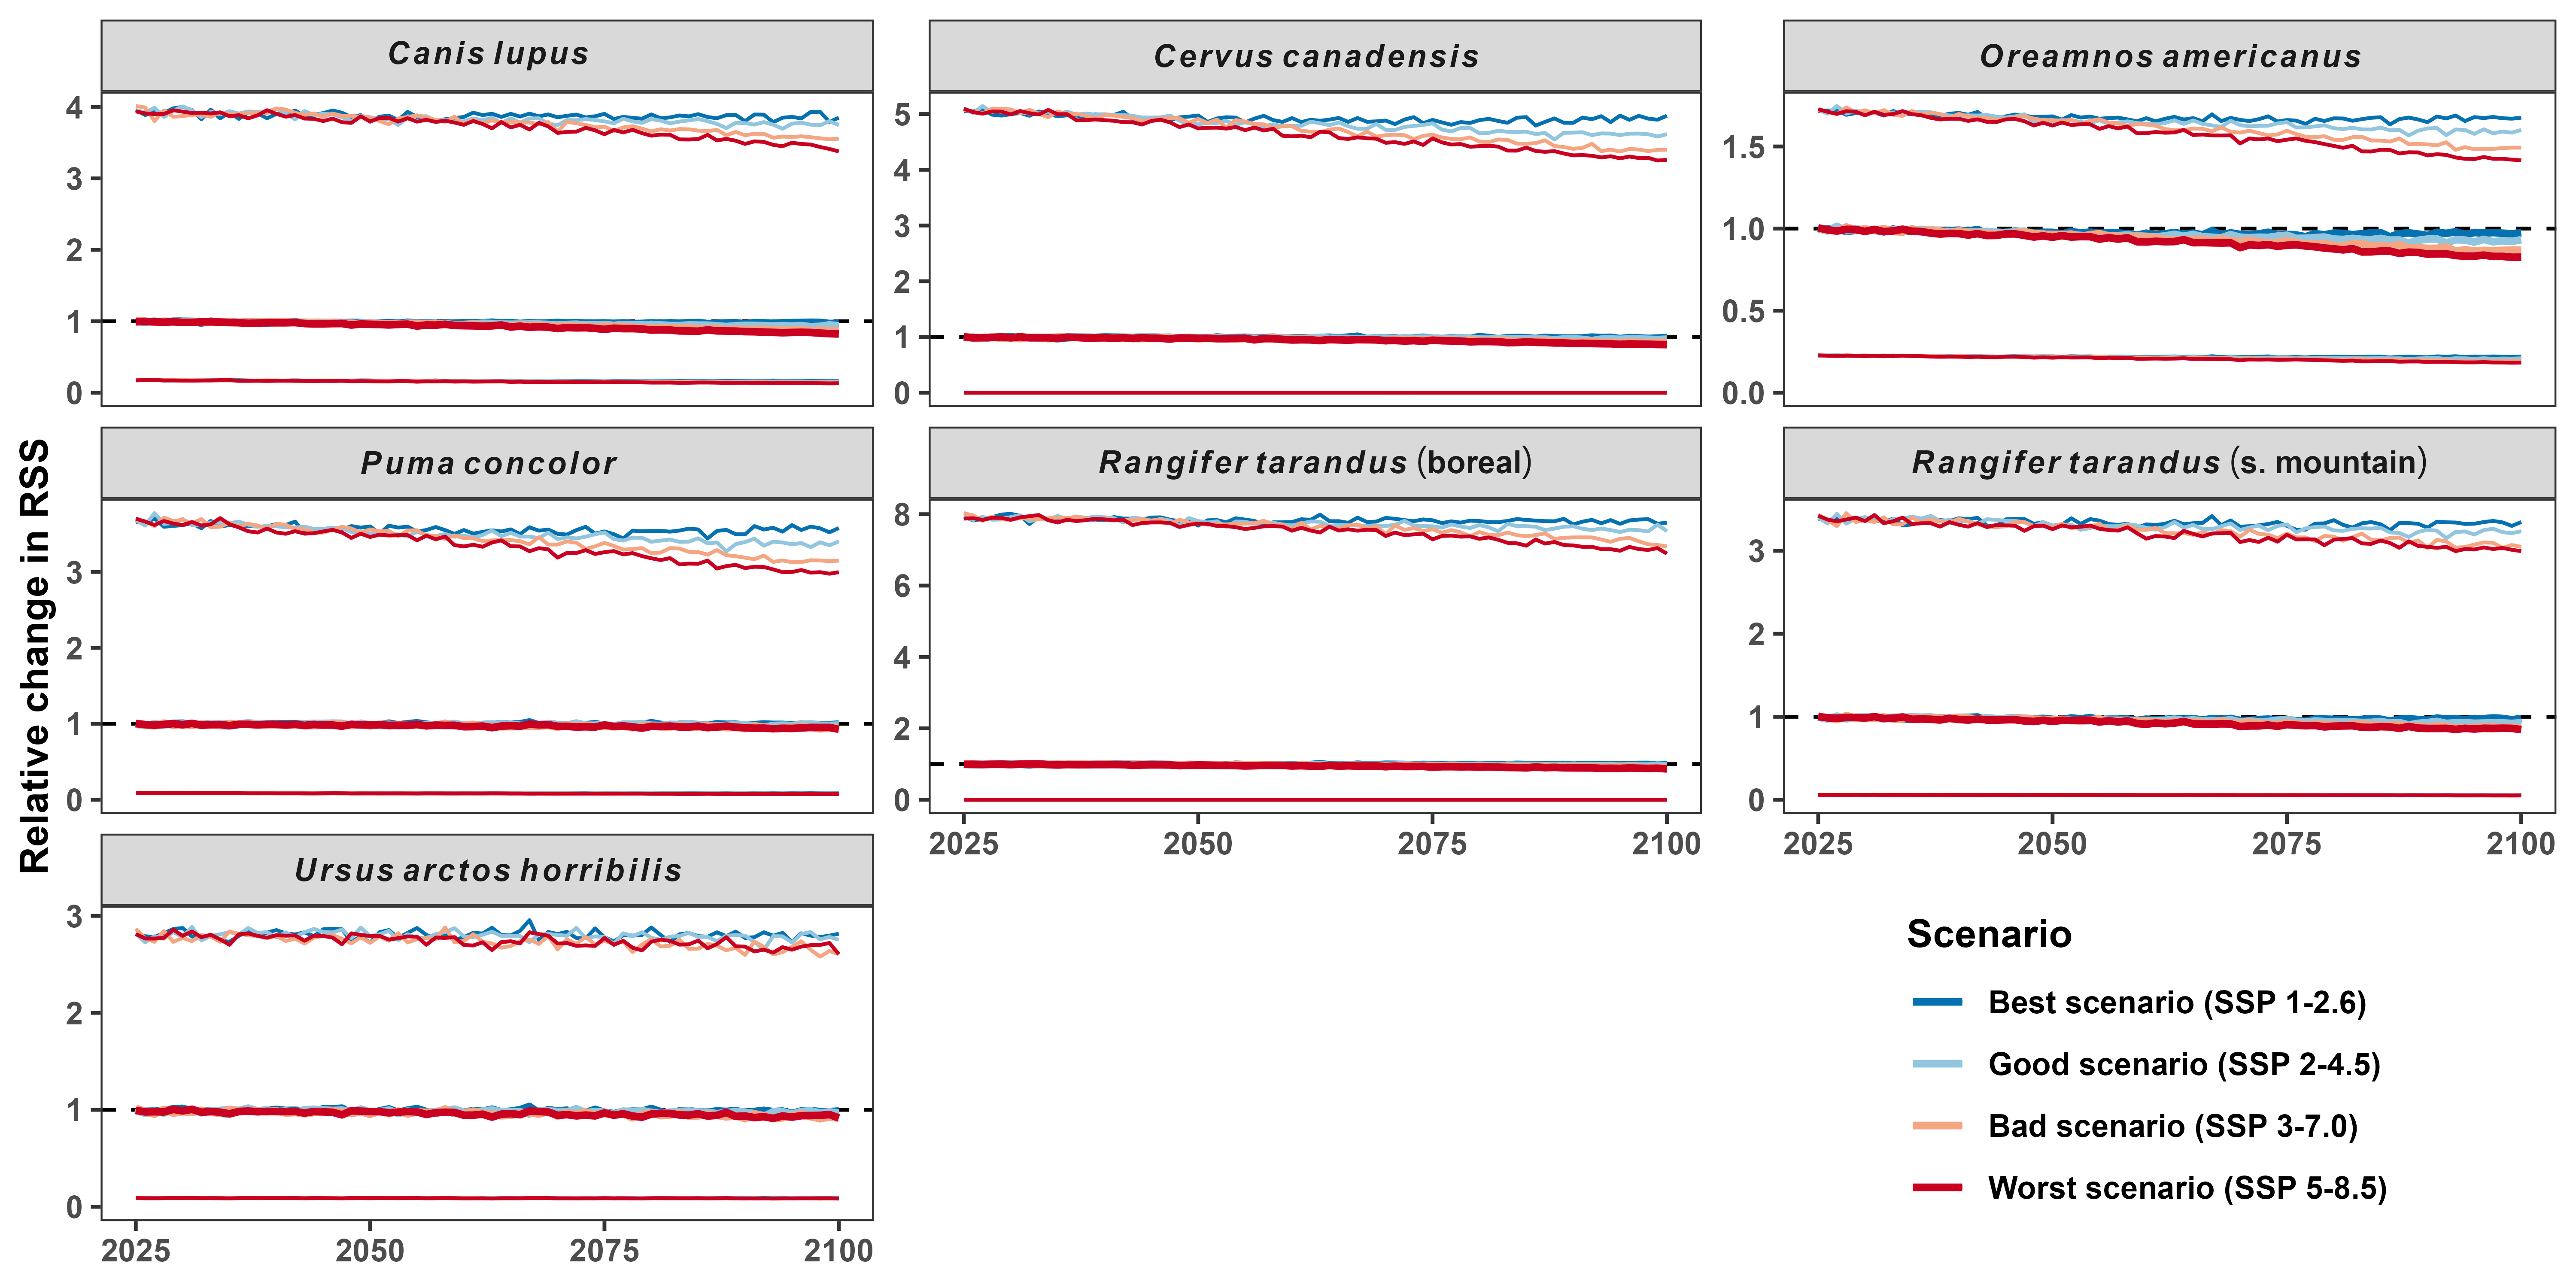
\includegraphics[width=\textwidth]{../figures/rss-local-cc-predictions} 

}

\caption{\textbf{Species are predicted to alter their habitat selection differently in response to climate change, and worse climate-change scenarios will result in the greatest change.} Bold lines indicate the change in median RSS due to predicted changes in temperature within each species' sutdy area. Shaded areas indicate the $95^\text{th}$ and $5^\text{th}$ percentiles in change in RSS. Values > 1 indicate an increase, while values < 1 indicate a decrease. Changes are relative to each location's mean RSS in 2025, averaged across the four Shared Socioeconomic Pathways (SSPs).}\label{fig:t-rss-cc}
\end{figure}

\begin{figure}

{\centering \includegraphics[width=\textwidth]{../figures/local-rss-2100} 

}

\caption{\textbf{Climate change will impact each species' relative selection strength (RSS) differently.} The color scale indicates the predicted changes in RSS in 2100, relative to each location's average RSS in 2025 across all four scenarios (i.e., not relative to other pixels). Values < 1 indicate a decrease and values > 1 indicate an increase. For ease of readability, the color bar is on the $\log_2$ scale to help visualize patterns in doubling, and values are capped to 0.8 and 1.25 ($\approx 2^{\pm 0.322}$; original data ranged 0.71 to 1.93). All maps extend to each species' study area and are shown in the BC Albers Equal Area Conic projection (EPSG:3005).}\label{fig:s-rss-cc}
\end{figure}

\begin{figure}

{\centering 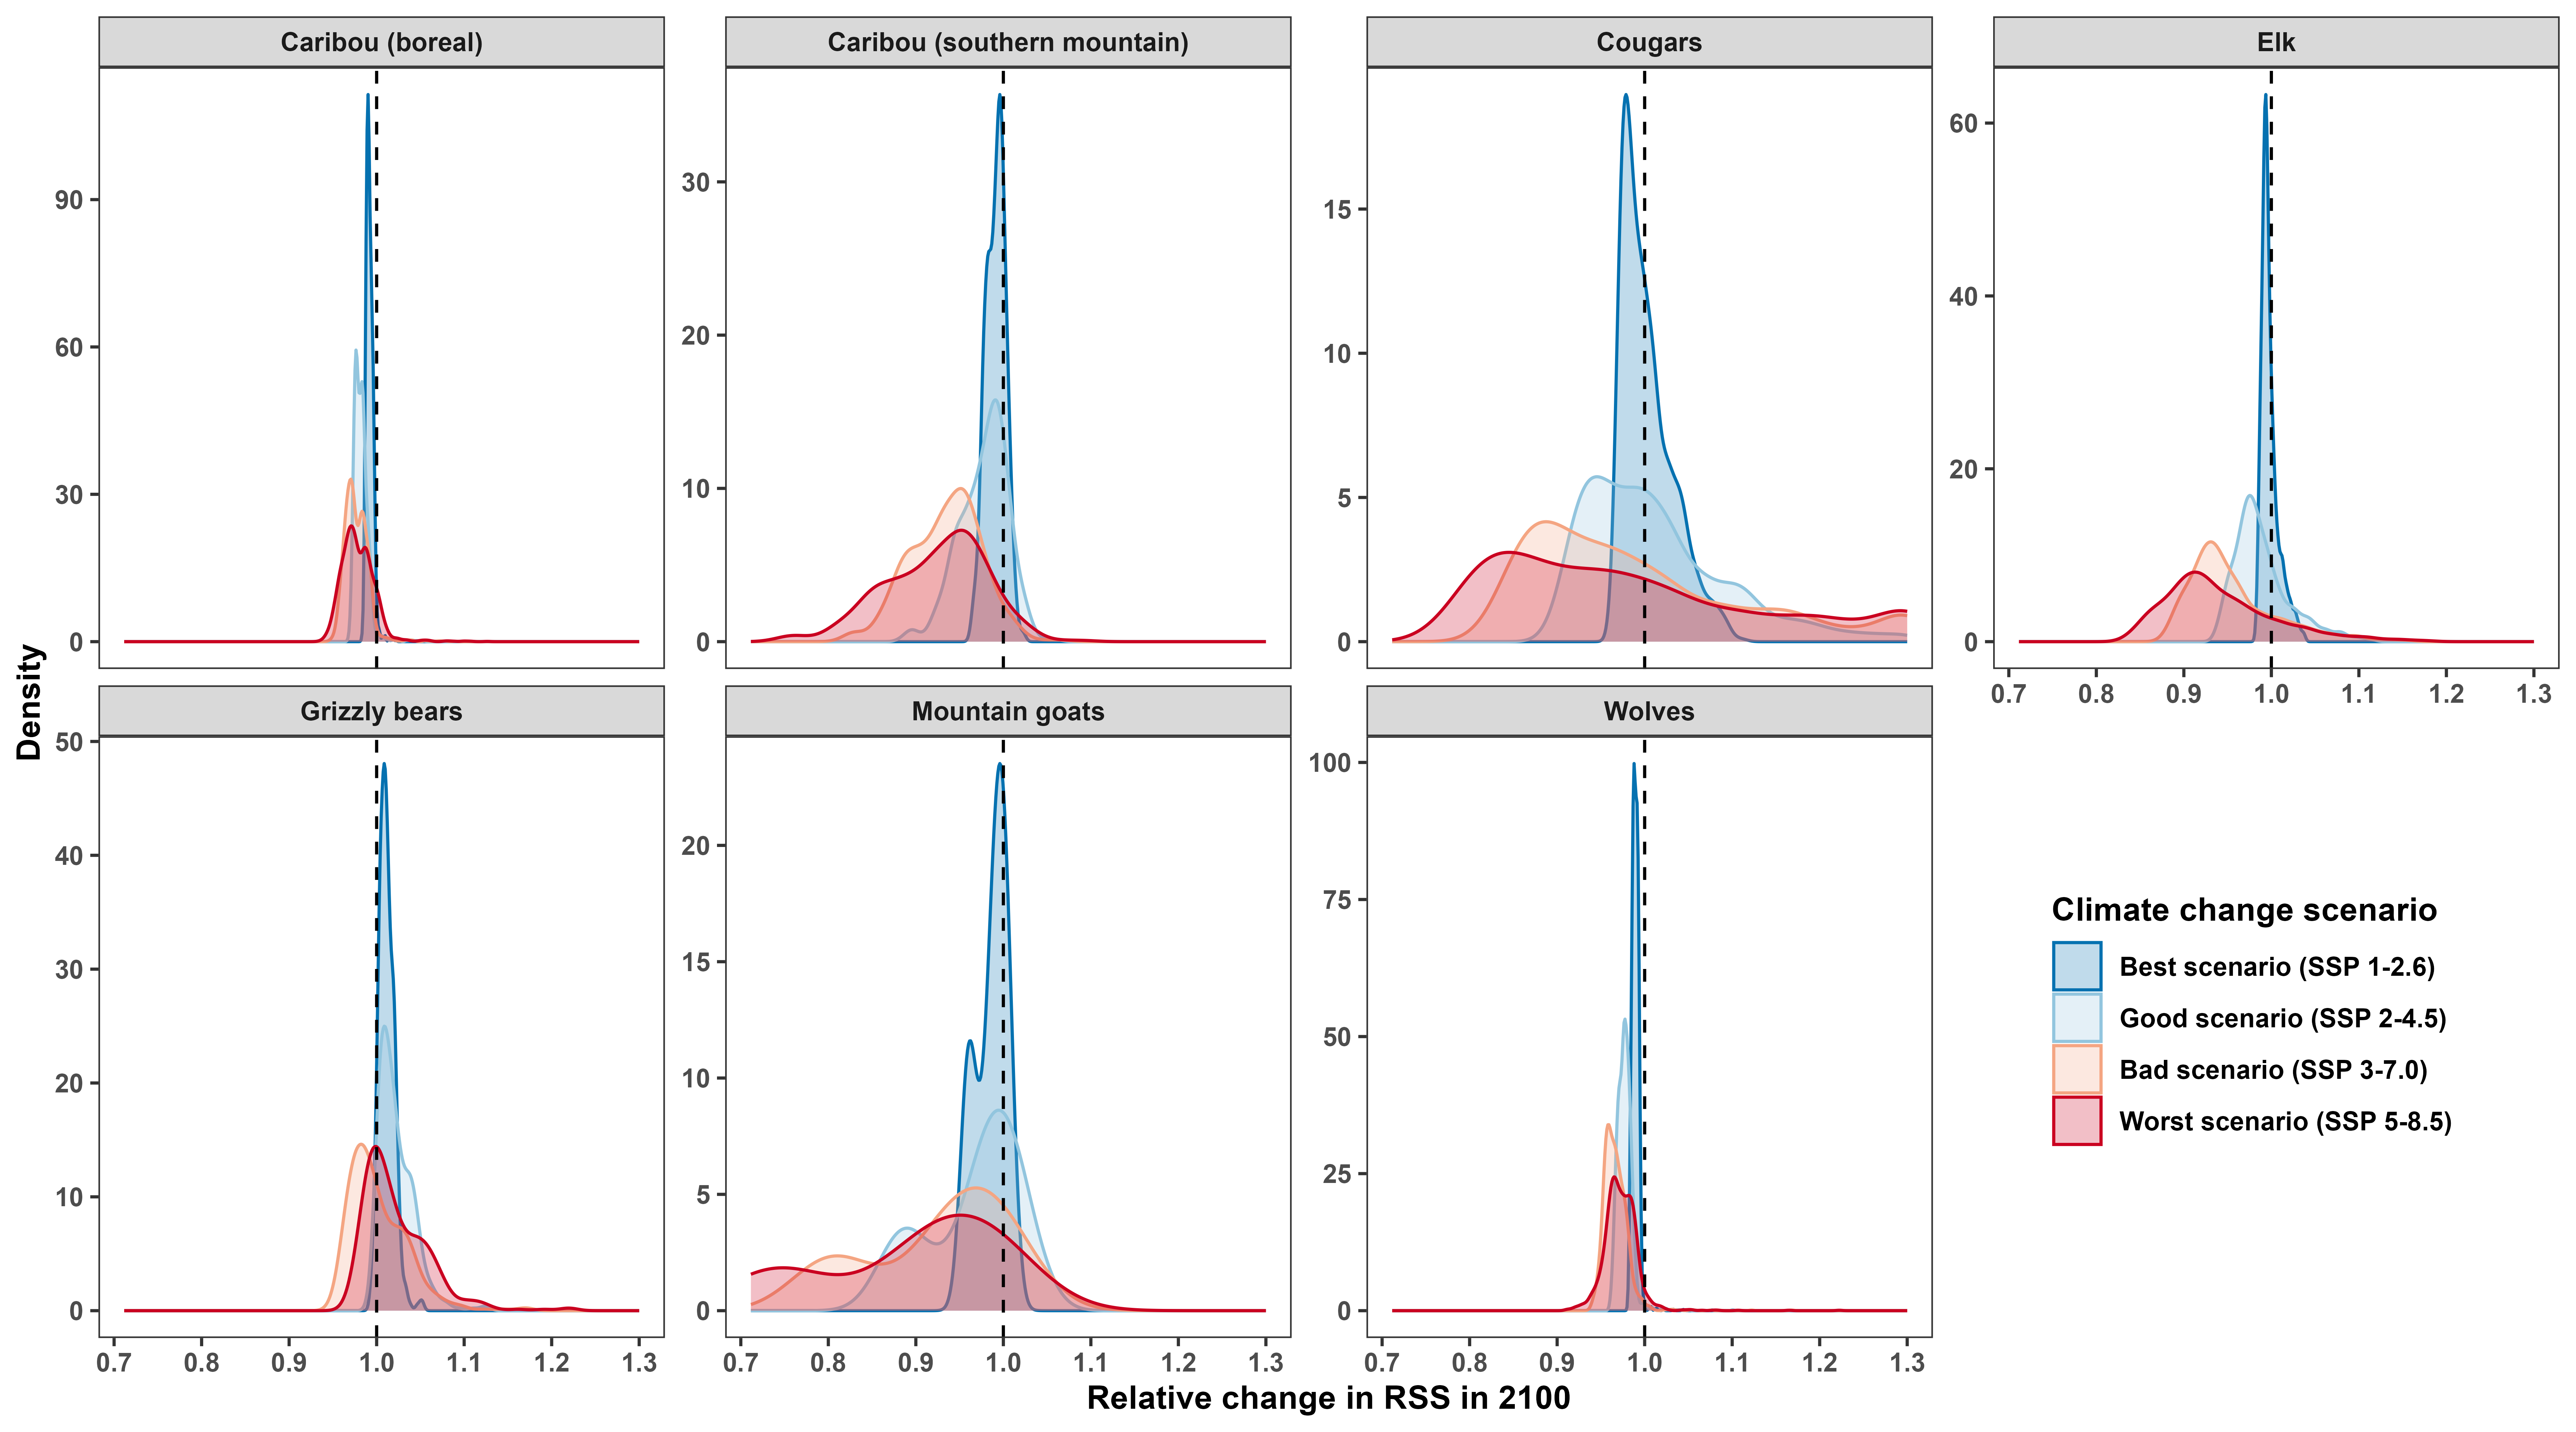
\includegraphics[width=\textwidth]{../figures/local-rss-2100-density} 

}

\caption{\textbf{Climate change is predicted to cause species to decrease their selection strength for their current habitats, and worse climate change scenarios will have the greatest impact.} The density plots indicate each species' change in RSS in 2100 for their current habitat (Fig. 8), relative to each location's RSS in 2025. Values < 1 indicate a decrease and values > 1 indicate an increase. For ease of readability, values > 1.3 were changed to 1.3 (original maximum: 1.93).}\label{fig:density-hrsfs}
\end{figure}

\section{Discussion}\label{discussion}

\noindent We have demonstrated that temperature is an important driver of how and where large temperate and Nearctic mammals move, affecting individuals' seasonal and daily movement behaviour in both non-linear, and species-specific ways. These findings are consistent with the broader recognition that behavioural responses to temperature vary substantially across species (McCain \& King, 2014; Gibert \emph{et al.}, 2016; Williams \& Blois, 2018; Noonan \emph{et al.}, 2026), and build on it by quantifying these differential responses across a community of co-occurring predators, prey, and competitors. By leveraging the flexibility of HGAMs with tensor product interaction terms, we were able to disentangle the effects of temperature from circadian and seasonal behavioural cycles without imposing rigid assumptions about the shape of species' responses (Simpson, 2018, 2025; Pedersen \emph{et al.}, 2019), an approach that was essential for characterising how mammals behave at the extreme temperatures that are becoming increasingly frequent in western Canada (Thompson \emph{et al.}, 2022; Zhang \emph{et al.}, 2023a). Projecting these models into the future, we found that the species-specific nature of these responses to temperature has direct implications for how this community of large mammals will interact under climate change. While cougars, elk, and wolves are projected to move less by 2100, southern mountain caribou and mountain goats will move more. When these projections are viewed alongside the species-specific shifts in habitat selection, the temperature-induced changes in movement rates and spatial overlap are likely to reshape encounter rates across the community (Martinez-Garcia \emph{et al.}, 2020). Indeed, the four-fold increase in caribou-wolf co-occupancy between -20°C and 20°C illustrates how temperature can fundamentally alter predator-prey dynamics even before accounting for projected changes in movement rates.

Unsurprisingly, the effects of warming temperatures on movement rates varied across species, reflecting species-specific differences in behaviour, physiology, and habitat use. For boreal caribou, we found that hotter temperatures decreased movement rates in summer but increased them in other seasons. These findings are consistent with previous studies (Stien \emph{et al.}, 2012; Leclerc \emph{et al.}, 2021; Lessard \emph{et al.}, 2025) and likely represent the outcome of two distinct mechanisms. In particular, the increase in movement rates with temperature during colder months is likely due in part to shallower snow depth, which increases mobility (Pedersen \emph{et al.}, 2021; Sullender \emph{et al.}, 2023), although we note that warmer temperatures during snowy seasons also increase the risk of rain-on-snow events (Musselman \emph{et al.}, 2018), which limit forage availability and increase time spent foraging (Stien \emph{et al.}, 2012; Berger \emph{et al.}, 2018). In contrast, the negative effect of temperature on movement during summer is likely due to the need for more frequent resting and use of thermal refugia, consistent with ungulates' documented risk of hyperthermia (Alston \emph{et al.}, 2020; Verzuh \emph{et al.}, 2023). The net result of these seasonal differences is that caribou yearly average movement rates were projected to remain approximately unchanged throughout the 21\textsuperscript{st} century. However, these coarse-grained annual averages mask potentially substantial shifts in seasonal movement phenology. The effects of these temporally dynamic responses to temperature may be exacerbated by mismatches with seasonal photoperiod (Walker \emph{et al.}, 2019), including the timing of molting and reproduction. Indeed, earlier growth seasons in boreal regions have resulted in lower calf birth and survival (Post \& Forchhammer, 2008), while the lengthening of the growth season has allowed moose (\emph{Alces alces}) and deer to encroach on boreal caribou habitat (Dawe \& Boutin, 2016) and increase the density of coyotes (\emph{Canis latrans}), cougars, and wolves (Barber \emph{et al.}, 2018; DeMars \emph{et al.}, 2023), whose movement behaviour also depends on ambient temperature. We found that wolves responded to temperature similarly to boreal caribou in terms of seasonal patterns, and their habitat selection strength was not projected to change markedly by 2100, yet they were still predicted to move less overall in future decades. In contrast, cougars showed the strongest and most consistent response across seasons, with warmer temperatures reducing travel regardless of time of year, producing the largest projected decrease in yearly movement rates of any species in this study, approximately 24\% by 2100 under the worst-case SSP. Similarly to boreal caribou, mountain goats' lower movement rates near 0°C in winter likely reflect multiple concurrent pressures, including increased energetic costs of movement through melting snow and rain-on-snow conditions (Musselman \emph{et al.}, 2018; White, 2025) and increased predation risk (Sullender \emph{et al.}, 2023), while milder temperatures increase plant growth and allow goats to spend more time foraging within rather than traveling between patches (Charnov, 1976; White \emph{et al.}, 2025), consistent with their projected increase in movement by 2100. Besides the changes in activity and movement rates, the species-specific shifts in habitat selection we document here are equally important for understanding how climate change will alter animals' spatial distributions. Across all species, the direction and magnitude of projected changes in habitat selection strength varied substantially, with RSS declining throughout most of each species' current range under all SSPs, most severely for elk, mountain goats, cougars, and southern mountain caribou. However, the spatial heterogeneity in projected RSS change highlights how the consequences of temperature-dependent habitat selection will not be uniformly distributed across the landscape.

Our caribou-wolf co-occupancy results are a prime example of how species-specific changes in movement and habitat selection can cascade to the community level. More specifically, we found that warmer temperatures cause both wolves and boreal caribou to increase their movement rates in fall, winter, and spring. In tandem with these changes in activity, warmer temperatures were found to increase the spatial overlap wolves and boreal caribou. Given the well-known importance of movement speed and spatial overlap on driving encounter rates (Gurarie \& Ovaskainen, 2013; Martinez-Garcia \emph{et al.}, 2020; Noonan \emph{et al.}, 2021), these trends suggest that warming temperatures may intensify the predation pressure on boreal caribou during periods when they are most vulnerable, including pregnancy and early calf-rearing. The four-fold increase in caribou-wolf co-occupancy between -20°C and 20°C illustrates the magnitude of these shifts in spatial overlap, and underscores that temperature-driven changes in encounter rates can be substantial even before accounting for projected changes in movement rates over the coming decades. Additionally, while both species saw reduced movement rates during hot summer days, wolves' use of anthropogenic linear features (e.g., roads, seismic lines) may allow them to reduce the total thermal costs of movement by moving for shorter periods while increasing the chances of encountering heat-stressed prey (Whittington \emph{et al.}, 2011; Dickie \emph{et al.}, 2017; Dickie \emph{et al.}, 2022). Crucially, caribou that attempt to reduce predation risk from wolves by avoiding wolf habitat may still risk increasing predation pressure from bears, cougars, and coyote (Leblond \emph{et al.}, 2016; DeMars \emph{et al.}, 2023; Labadie \emph{et al.}, 2023). Beyond changes in movement rates, the projected declines in RSS across most species' current ranges, combined with the tendency for elk, mountain goats, and cougars to shift toward higher elevations as temperatures warm, will concentrate multiple species in shrinking areas of suitable habitat, further increasing encounter rates among competitors and between predators and prey (Kohl \emph{et al.}, 2019; Martinez-Garcia \emph{et al.}, 2020). Together, these findings suggest that the community-level consequences of climate change will be driven not just by how individual species respond to warming, but by how those responses interact across trophic levels to reshape the spatial structure of the entire community.

Considerations about changes in trophic interactions lead to an important caveat: The climate change projections we present here account only for the direct effects of changing temperature on movement behaviour. This is almost certainly an oversimplification of how these species, and landscapes through which they move will change over the coming decades. For example, climate change has already driven widespread shifts in plant phenology and productivity across western Canada (Cleland \emph{et al.}, 2007; Denny, 2019; Tysor, 2025), with consequences for the distribution and timing of forage that herbivores depend on (Post \& Forchhammer, 2008; Aikens \emph{et al.}, 2017). Plants' limited capacity to disperse to and establish in new areas means that herbivores shifting to higher elevations in response to warming may outpace the plant communities they rely on (Speed \emph{et al.}, 2012; Diffenbaugh \& Field, 2013), forcing individuals to spend more time traveling between patches and increasing both energetic expenditure and exposure to predators (Kohl \emph{et al.}, 2019; Martinez-Garcia \emph{et al.}, 2020; Mezzini \emph{et al.}, 2025). The spatial heterogeneity in projected RSS declines we document (Fig. \ref{fig:s-rss-cc}) suggests that these dynamics will be particularly acute in areas where suitable high-elevation habitat is isolated, since species seeking thermal refuge will be forced to traverse intervening areas of low habitat quality and elevated predation risk (Lamb \emph{et al.}, 2025; White \emph{et al.}, 2025). Furthermore, forests in western Canada are highly dynamic (Zhang \emph{et al.}, 2015), and fire size and burn severity have increased markedly in recent decades (Whitman \emph{et al.}, 2022; Parisien \emph{et al.}, 2023; Wang \emph{et al.}, 2025). Our use of a static forest cover raster was a pragmatic modelling choice that facilitated straightforward climate change projections, but future work should account for how fire, logging, and other drivers of forest change will interact with temperature to shape mammalian movement behaviour and habitat selection (Dickie \emph{et al.}, 2017, 2024; Lochhead \emph{et al.}, 2022). The results presented here are therefore best interpreted as an `all-else-being-equal' baseline that captures the direct behavioural responses to temperature while holding the landscape constant. The true community-level consequences of climate change will be more complex than our projections alone suggest.

While this work represents an important step forward towards understanding the community-level consequences of species-specific responses to climate change, several limitations of our approach warrant consideration. First, the estimated effects of temperature on movement behaviour cannot be fully attributed to direct physiological responses to temperature alone, since temperature is non-linearly correlated with other aspects of seasonal phenology that independently drive movement decisions (\emph{sensu} Nathan \emph{et al.}, 2008). Our findings for mountain goats are a clear illustration of this point. Their lower movement rates near 0°C in winter could reflect increased energetic costs of movement through melting snow and rain-on-snow conditions (White, 2025), reduced movement during storms (Musselman \emph{et al.}, 2018), increased predation risk (Sullender \emph{et al.}, 2023), or some combination of these factors, all of which co-vary with temperature. The smooth functions estimated by our HGAMs capture the total effect of temperature on movement behaviour, including both direct physiological effects and indirect effects mediated through correlated variables, and should be interpreted accordingly. Second, the habitat selection models we present are based on three broadly applicable covariates chosen for their relevance to thermoregulation across a taxonomically diverse community (Dobrowski, 2011; McLaughlin \emph{et al.}, 2017; Attias \emph{et al.}, 2018; McCain, 2019; Stralberg \emph{et al.}, 2020; Fuller \emph{et al.}, 2021; Giroux \emph{et al.}, 2023; Verzuh \emph{et al.}, 2023; Zhang \emph{et al.}, 2023b; Noonan \emph{et al.}, 2026), but forest cover, elevation, and distance from water are often correlated, and the estimated selection coefficients may not be transferable outside the study areas used here. For example, both mountain goats and elk selected for higher elevation as temperatures warmed, but our models did not account for differences in forage availability at different elevations, which may confound the interpretation of elevational selection in areas with different vegetation.

Temperature is not the only driver of mammalian movement (Nathan \emph{et al.}, 2008), but it is an important one (McCain \& King, 2014; Williams \& Blois, 2018; Noonan \emph{et al.}, 2026). Warming temperatures are shaping not only how and where individual species move, but can have cascading influences on how co-occurring species interact across trophic levels (Latham \emph{et al.}, 2011; Creel \emph{et al.}, 2016; Bastille-Rousseau \emph{et al.}, 2018; Labadie \emph{et al.}, 2023; Sullender \emph{et al.}, 2023; Brivio \emph{et al.}, 2024; Carroll \emph{et al.}, 2024), stressing the existing balance between heat stress and predator avoidance (Milling \emph{et al.}, 2017). Concurrently, growing human presence and landscape transformation have had substantial effects on animals' movement rates and behaviour (Sih \emph{et al.}, 2011; Tucker \emph{et al.}, 2018) as well as the occurrence of predator-prey interactions (Whittington \emph{et al.}, 2011; Dickie \emph{et al.}, 2017) and human-wildlife interactions (Johnson \emph{et al.}, 2018; Rabaiotti \emph{et al.}, 2021; Balyx, 2022; Abrahms \emph{et al.}, 2023; Weststrate \emph{et al.}, 2024; Lamb \emph{et al.}, 2025; Lessard \emph{et al.}, 2025). By quantifying the effects of temperature on movement rates and habitat selection effects simultaneously across a community of predators, prey, and competitors, we have shown that the species-specific and non-linear nature of thermal responses will drive complex changes in movement rates and habitat selection under climate change, with cascading consequences for the encounter rates that govern predator-prey dynamics, competitive interactions, and community structure (Gurarie \& Ovaskainen, 2013; Martinez-Garcia \emph{et al.}, 2020; Noonan \emph{et al.}, 2021). The four-fold increase in caribou-wolf co-occupancy driven by temperature alone highlights how substantial these community-level consequences can be, and our projections suggest they will only intensify as temperatures continue to rise throughout the 21st century (IPCC, 2023). Critically, because responses to warming were species-specific, the community-level consequences of climate change cannot be anticipated from single-species approaches alone (Gibert \emph{et al.}, 2016; Cunningham \emph{et al.}, 2021). In this context, the hierarchical GAM framework we employed provides a flexible and broadly applicable tool for characterising these complex, nonlinear responses across multiple species simultaneously (Polazzo \emph{et al.}, 2024), and we encourage its application to other communities where the ecological consequences of climate change remain poorly understood (Cunningham \emph{et al.}, 2021). Ultimately, anticipating how warming temperatures will restructure ecological communities requires moving beyond the question of how individual species will respond to change, toward an understanding of how those responses will interact across trophic levels to reshape the spatial and temporal structure of the communities they form.

\section*{Acknowledgements}\label{acknowledgements}
\addcontentsline{toc}{section}{Acknowledgements}

\noindent We would like to thank Kirk Safford from the British Columbia Ministry of Environment and Parks (BC Parks) in Penticton, BC, Canada for providing the mountain goat telemetry data. SM would also like to thank BC Parks and Biodiversity Pathways for financial suppport, and also all those who provided feedback following presentations and poster sessions.

\section*{Author contributions}\label{author-contributions}
\addcontentsline{toc}{section}{Author contributions}

\noindent SM performed the data cleaning, ran the analyses, and wrote the manuscript. CHF wrote code for estimating instantaneous movement speeds. MJN conceived of the project idea and supervised SM throughout the project. All other authors contributed telemetry data and/or reviewed the interpretation of the results for their species of interest. KH and SD contributed substantially to manuscript review. All authors contributed to reviewing the manuscript.

\clearpage

\newpage

\section*{References}\label{references}
\addcontentsline{toc}{section}{References}

\hangparas{1em}{1}

\phantomsection\label{refs}
\begin{CSLReferences}{1}{0}
\bibitem[\citeproctext]{ref-aarts_estimating_2008}
Aarts G, MacKenzie M, McConnell B, Fedak M, Matthiopoulos J (2008) \href{https://doi.org/10.1111/j.2007.0906-7590.05236.x}{Estimating space-use and habitat preference from wildlife telemetry data}. \emph{Ecography}, \textbf{31}, 140--160.

\bibitem[\citeproctext]{ref-abrahms_climate_2023}
Abrahms B, Carter NH, Clark-Wolf TJ et al. (2023) \href{https://doi.org/10.1038/s41558-023-01608-5}{Climate change as a global amplifier of human--wildlife conflict}. \emph{Nature Climate Change}, \textbf{13}, 224--234.

\bibitem[\citeproctext]{ref-aikens_greenscape_2017}
Aikens EO, Kauffman MJ, Merkle JA, Dwinnell SPH, Fralick GL, Monteith KL (2017) \href{https://doi.org/10.1111/ele.12772}{The greenscape shapes surfing of resource waves in a large migratory herbivore} (ed Nathan R). \emph{Ecology Letters}, \textbf{20}, 741--750.

\bibitem[\citeproctext]{ref-aikens_pronghorn_2025}
Aikens EO, Merkle JA, Xu W, Sawyer H (2025) Pronghorn movements and mortality during extreme weather highlight the critical importance of connectivity. \emph{Current Biology}, \textbf{35}, 1927--1934.

\bibitem[\citeproctext]{ref-alston_temperature_2020}
Alston JM, Joyce MJ, Merkle JA, Moen RA (2020) \href{https://doi.org/10.1007/s10980-020-01072-y}{Temperature shapes movement and habitat selection by a heat-sensitive ungulate}. \emph{Landscape Ecology}, \textbf{35}, 1961--1973.

\bibitem[\citeproctext]{ref-alston_mitigating_2022}
Alston JM, Fleming CH, Kays R et al. (2022) \href{https://doi.org/10.1111/2041-210X.14025}{Mitigating pseudoreplication and bias in resource selection functions with autocorrelation‐informed weighting}. \emph{Methods in Ecology and Evolution}, 2041--210X.14025.

\bibitem[\citeproctext]{ref-arechavala-lopez_common_2019}
Arechavala-Lopez P, Minguito-Frutos M, Follana-Berná G, Palmer M (2019) \href{https://doi.org/10.1093/icesjms/fsy014}{Common octopus settled in human-altered {Mediterranean} coastal waters: From individual home range to population dynamics} (ed Durif C). \emph{ICES Journal of Marine Science}, \textbf{76}, 585--597.

\bibitem[\citeproctext]{ref-attias_effects_2018}
Attias N, Oliveira-Santos LGR, Fagan WF, Mourão G (2018) \href{https://doi.org/10.1016/j.anbehav.2018.04.011}{Effects of air temperature on habitat selection and activity patterns of two tropical imperfect homeotherms}. \emph{Animal Behaviour}, \textbf{140}, 129--140.

\bibitem[\citeproctext]{ref-baddeley_spatial_2015}
Baddeley A, Rubak E, Turner R (2015) \emph{\emph{\href{https://doi.org/10.1201/b19708}{Spatial {Point} {Patterns}: {Methodology} and {Applications} with {R}}}}, 0th edn. Chapman; Hall/CRC.

\bibitem[\citeproctext]{ref-balyx_human_2022}
Balyx L (2022) \href{https://doi.org/10.14288/1.0416294}{Human conflict and coexistence with mountain goats in a protected alpine landscape}.

\bibitem[\citeproctext]{ref-barber_potential_2018}
Barber QE, Parisien M, Whitman E et al. (2018) \href{https://doi.org/10.1002/ecs2.2472}{Potential impacts of climate change on the habitat of boreal woodland caribou}. \emph{Ecosphere}, \textbf{9}, e02472.

\bibitem[\citeproctext]{ref-bastille-rousseau_climate_2018}
Bastille-Rousseau G, Schaefer JA, Peers MJL et al. (2018) \href{https://doi.org/10.1007/s00442-017-4017-y}{Climate change can alter predator--prey dynamics and population viability of prey}. \emph{Oecologia}, \textbf{186}, 141--150.

\bibitem[\citeproctext]{ref-basu_phenological_2024}
Basu A, Culpepper J, Blagrave K, Sharma S (2024) \href{https://doi.org/10.1029/2023WR036392}{Phenological {Shifts} in {Lake} {Ice} {Cover} {Across} the {Northern} {Hemisphere}: {A} {Glimpse} {Into} the {Past}, {Present}, and the {Future} of {Lake} {Ice} {Phenology}}. \emph{Water Resources Research}, \textbf{60}, e2023WR036392.

\bibitem[\citeproctext]{ref-bc_ogris_boreal_2018}
BC OGRIS (2018) \href{https://www.bcogris.ca/projects/boreal-caribou-telemetry-data}{Boreal {Caribou} and {Wolf} {Telemetry} {Data}}.

\bibitem[\citeproctext]{ref-berger_climate_2018}
Berger J, Hartway C, Gruzdev A, Johnson M (2018) \href{https://doi.org/10.1038/s41598-018-19416-9}{Climate {Degradation} and {Extreme} {Icing} {Events} {Constrain} {Life} in {Cold}-{Adapted} {Mammals}}. \emph{Scientific Reports}, \textbf{8}, 1156.

\bibitem[\citeproctext]{ref-bird_cougar_2010}
Bird C, Clarke R, Lewis D, Serrouya R (2010) Cougar ecology, predation, and caribou in the {Columbia} {Mountains} of {British} {Columbia}. \emph{Fish and Wildlife Compensation Program}.

\bibitem[\citeproctext]{ref-blanchong_respiratory_2018}
Blanchong JA, Anderson CA, Clark NJ et al. (2018) \href{https://doi.org/10.1002/jwmg.21470}{Respiratory disease, behavior, and survival of mountain goat kids}. \emph{The Journal of Wildlife Management}, \textbf{82}, 1243--1251.

\bibitem[\citeproctext]{ref-botero_evolutionary_2015}
Botero CA, Weissing FJ, Wright J, Rubenstein DR (2015) \href{https://doi.org/10.1073/pnas.1408589111}{Evolutionary tipping points in the capacity to adapt to environmental change}. \emph{Proceedings of the National Academy of Sciences}, \textbf{112}, 184--189.

\bibitem[\citeproctext]{ref-brivio_seeking_2024}
Brivio F, Apollonio M, Anderwald P, Filli F, Bassano B, Bertolucci C, Grignolio S (2024) \href{https://doi.org/10.1098/rspb.2023.1587}{Seeking temporal refugia to heat stress: Increasing nocturnal activity despite predation risk}. \emph{Proceedings of the Royal Society B: Biological Sciences}, \textbf{291}, 20231587.

\bibitem[\citeproctext]{ref-brown_toward_2004}
Brown JH, Gillooly JF, Allen AP, Savage VM, West GB (2004) \href{https://doi.org/10.1890/03-9000}{Toward a metabolic theory of ecology}. \emph{Ecology}, \textbf{85}, 1771--1789.

\bibitem[\citeproctext]{ref-buderman_time-varying_2018}
Buderman FE, Hooten MB, Alldredge MW, Hanks EM, Ivan JS (2018) \href{https://doi.org/10.1186/s40462-018-0140-6}{Time-varying predatory behavior is primary predictor of fine-scale movement of wildland-urban cougars}. \emph{Movement Ecology}, \textbf{6}, 22.

\bibitem[\citeproctext]{ref-bunnell_global_2011}
Bunnell FL, Kremsater LL, Wells RW (2011) \href{https://doi.org/10.22230/jem.2011v12n2a74}{Global {Weirding} in {British} {Columbia}: {Climate} {Change} and the {Habitat} of {Terrestrial} {Vertebrates}}. \emph{Journal of Ecosystems and Management}, \textbf{12}.

\bibitem[\citeproctext]{ref-burnett_climatenar_2023}
Burnett M (2023) \emph{\emph{{climatenaR}: {Tools} to {Access} {ClimateNA} data}}.

\bibitem[\citeproctext]{ref-calabrese_ctmm_2016}
Calabrese JM, Fleming CH, Gurarie E (2016) \href{https://doi.org/10.1111/2041-210X.12559}{Ctmm: An {R} package for analyzing animal relocation data as a continuous‐time stochastic process} (ed Freckleton R). \emph{Methods in Ecology and Evolution}, \textbf{7}, 1124--1132.

\bibitem[\citeproctext]{ref-carbeck_adaptation_2022}
Carbeck K, Wang T, Reid JM, Arcese P (2022) \href{https://doi.org/10.1111/gcb.16185}{Adaptation to climate change through seasonal migration revealed by climatic versus demographic niche models}. \emph{Global Change Biology}, \textbf{28}, 4260--4275.

\bibitem[\citeproctext]{ref-carroll_spatial_2024}
Carroll G, Abrahms B, Brodie S, Cimino MA (2024) \href{https://doi.org/10.1038/s41559-024-02454-0}{Spatial match--mismatch between predators and prey under climate change}. \emph{Nature Ecology \& Evolution}, \textbf{8}, 1593--1601.

\bibitem[\citeproctext]{ref-charnov_optimal_1976}
Charnov EL (1976) \href{https://doi.org/10.1016/0040-5809(76)90040-X}{Optimal foraging, the marginal value theorem}. \emph{Theoretical Population Biology}, \textbf{9}, 129--136.

\bibitem[\citeproctext]{ref-ciuti_human_2012}
Ciuti S, Muhly TB, Paton DG, McDevitt AD, Musiani M, Boyce MS (2012) \href{https://doi.org/10.1098/rspb.2012.1483}{Human selection of elk behavioural traits in a landscape of fear}. \emph{Proceedings of the Royal Society B: Biological Sciences}, \textbf{279}, 4407--4416.

\bibitem[\citeproctext]{ref-cleland_shifting_2007}
Cleland E, Chuine I, Menzel A, Mooney H, Schwartz M (2007) \href{https://doi.org/10.1016/j.tree.2007.04.003}{Shifting plant phenology in response to global change}. \emph{Trends in Ecology \& Evolution}, \textbf{22}, 357--365.

\bibitem[\citeproctext]{ref-creel_hunting_2016}
Creel S, Creel NM, Creel AM, Creel BM (2016) \href{https://doi.org/10.1002/ecy.1568}{Hunting on a hot day: Effects of temperature on interactions between {African} wild dogs and their prey}. \emph{Ecology}, \textbf{97}, 2910--2916.

\bibitem[\citeproctext]{ref-cunningham_opportunity_2021}
Cunningham SJ, Gardner JL, Martin RO (2021) \href{https://doi.org/10.1002/fee.2324}{Opportunity costs and the response of birds and mammals to climate warming}. \emph{Frontiers in Ecology and the Environment}, \textbf{19}, 300--307.

\bibitem[\citeproctext]{ref-darlington_southern_2025}
Darlington S, Gooliaff T, Stent P, Hodges K, Ford AT (2025) Southern {BC} {Cougar} {Project}. {Movebank} study 1620039803.

\bibitem[\citeproctext]{ref-dawe_climate_2016}
Dawe KL, Boutin S (2016) \href{https://doi.org/10.1002/ece3.2316}{Climate change is the primary driver of white‐tailed deer ( \emph{{Odocoileus} virginianus} ) range expansion at the northern extent of its range; land use is secondary}. \emph{Ecology and Evolution}, \textbf{6}, 6435--6451.

\bibitem[\citeproctext]{ref-deb_modelling_2020}
Deb JC, Forbes G, MacLean DA (2020) \href{https://doi.org/10.1111/mam.12210}{Modelling the spatial distribution of selected {North} {American} woodland mammals under future climate scenarios}. \emph{Mammal Review}, \textbf{50}, 440--452.

\bibitem[\citeproctext]{ref-demars_incorporating_2023}
DeMars CA, Johnson CJ, Dickie M et al. (2023) \href{https://doi.org/10.1002/ecs2.4627}{Incorporating mechanism into conservation actions in an age of multiple and emerging threats: {The} case of boreal caribou}. \emph{Ecosphere}, \textbf{14}, e4627.

\bibitem[\citeproctext]{ref-denicola_are_2025}
DeNicola VL, Mezzini S, Cagnacci F, Fleming CH (2025) \href{https://doi.org/10.1101/2025.07.17.665364}{Are your data too coarse for speed estimation? {Diffusion} rates as an alternative measure of animal movement}.

\bibitem[\citeproctext]{ref-denny_performance_2019}
Denny M (2019) \href{https://doi.org/10.1093/conphys/coz053}{Performance in a variable world: Using {Jensen}'s inequality to scale up from individuals to populations} (ed Domenici P). \emph{Conservation Physiology}, \textbf{7}, coz053.

\bibitem[\citeproctext]{ref-dickie_faster_2017}
Dickie M, Serrouya R, McNay RS, Boutin S (2017) \href{https://doi.org/10.1111/1365-2664.12732}{Faster and farther: Wolf movement on linear features and implications for hunting behaviour} (ed Du Toit J). \emph{Journal of Applied Ecology}, \textbf{54}, 253--263.

\bibitem[\citeproctext]{ref-dickie_resource_2022}
Dickie M, Serrouya R, Avgar T et al. (2022) \href{https://doi.org/10.1002/ecy.3642}{Resource exploitation efficiency collapses the home range of an apex predator}. \emph{Ecology}.

\bibitem[\citeproctext]{ref-dickie_habitat_2024}
Dickie M, Serrouya R, Becker M et al. (2024) \href{https://doi.org/10.1111/gcb.17286}{Habitat alteration or climate: {What} drives the densities of an invading ungulate?} \emph{Global Change Biology}, \textbf{30}, e17286.

\bibitem[\citeproctext]{ref-dierauer_climate_2021}
Dierauer JR, Allen DM, Whitfield PH (2021) \href{https://doi.org/10.1080/07011784.2021.1960894}{Climate change impacts on snow and streamflow drought regimes in four ecoregions of {British} {Columbia}}. \emph{Canadian Water Resources Journal / Revue canadienne des ressources hydriques}, \textbf{46}, 168--193.

\bibitem[\citeproctext]{ref-diffenbaugh_changes_2013}
Diffenbaugh NS, Field CB (2013) \href{https://doi.org/10.1126/science.1237123}{Changes in {Ecologically} {Critical} {Terrestrial} {Climate} {Conditions}}. \emph{Science}, \textbf{341}, 486--492.

\bibitem[\citeproctext]{ref-dobrowski_climatic_2011}
Dobrowski SZ (2011) \href{https://doi.org/10.1111/j.1365-2486.2010.02263.x}{A climatic basis for microrefugia: The influence of terrain on climate}. \emph{Global Change Biology}, \textbf{17}, 1022--1035.

\bibitem[\citeproctext]{ref-dougherty_going_2018}
Dougherty ER, Seidel DP, Carlson CJ, Spiegel O, Getz WM (2018) Going through the motions: Incorporating movement analyses into disease research. \emph{Ecology letters}, \textbf{21}, 588--604.

\bibitem[\citeproctext]{ref-dyer_travel_2023}
Dyer A, Brose U, Berti E, Rosenbaum B, Hirt MR (2023) \href{https://doi.org/10.1371/journal.pbio.3001820}{The travel speeds of large animals are limited by their heat-dissipation capacities} (ed Hedenström A). \emph{PLOS Biology}, \textbf{21}, e3001820.

\bibitem[\citeproctext]{ref-elmore_implications_2017}
Elmore RD, Carroll JM, Tanner EP, Hovick TJ, Grisham BA, Fuhlendorf SD, Windels SK (2017) \href{https://doi.org/10.1002/wsb.772}{Implications of the thermal environment for terrestrial wildlife management}. \emph{Wildlife Society Bulletin}, \textbf{41}, 183--193.

\bibitem[\citeproctext]{ref-fithian_finite-sample_2013}
Fithian W, Hastie T (2013) \href{https://doi.org/10.1214/13-AOAS667}{Finite-sample equivalence in statistical models for presence-only data}. \emph{The Annals of Applied Statistics}, \textbf{7}.

\bibitem[\citeproctext]{ref-fleming_ctmm_2023}
Fleming CH, Calabrese JM (2023) \emph{\emph{\href{https://CRAN.R-project.org/package=ctmm}{Ctmm: {Continuous}-{Time} {Movement} {Modeling}}}}.

\bibitem[\citeproctext]{ref-fleming_fine-scale_2014}
Fleming CH, Calabrese JM, Mueller T, Olson KA, Leimgruber P, Fagan WF (2014) \href{https://doi.org/10.1086/675504}{From {Fine}-{Scale} {Foraging} to {Home} {Ranges}: {A} {Semivariance} {Approach} to {Identifying} {Movement} {Modes} across {Spatiotemporal} {Scales}}. \emph{The American Naturalist}, \textbf{183}, E154--E167.

\bibitem[\citeproctext]{ref-ford_effects_2023}
Ford AT, Noonan MJ, Bollefer K, Gill R, Legebokow C, Serrouya R (2023) \href{https://doi.org/10.1111/acv.12801}{The effects of maternal penning on the movement ecology of mountain caribou}. \emph{Animal Conservation}, \textbf{26}, 72--85.

\bibitem[\citeproctext]{ref-fuller_towards_2016}
Fuller A, Mitchell D, Maloney SK, Hetem RS (2016) \href{https://doi.org/10.1186/s40665-016-0024-1}{Towards a mechanistic understanding of the responses of large terrestrial mammals to heat and aridity associated with climate change}. \emph{Climate Change Responses}, \textbf{3}, 10.

\bibitem[\citeproctext]{ref-fuller_how_2021}
Fuller A, Mitchell D, Maloney SK et al. (2021) \href{https://doi.org/10.1242/jeb.238113}{How dryland mammals will respond to climate change: The effects of body size, heat load and a lack of food and water}. \emph{Journal of Experimental Biology}, \textbf{224}, jeb238113.

\bibitem[\citeproctext]{ref-gibert_crossing_2016}
Gibert JP, Chelini M-C, Rosenthal MF, DeLong JP (2016) Crossing regimes of temperature dependence in animal movement. \emph{Global Change Biology}, \textbf{22}, 1722--1736.

\bibitem[\citeproctext]{ref-giroux_activity_2023}
Giroux A, Ortega Z, Attias N, Desbiez ALJ, Valle D, Börger L, Rodrigues Oliveira-Santos LG (2023) \href{https://doi.org/10.1016/j.anbehav.2023.04.008}{Activity modulation and selection for forests help giant anteaters to cope with temperature changes}. \emph{Animal Behaviour}, \textbf{201}, 191--209.

\bibitem[\citeproctext]{ref-guiden_seasonal_2020}
Guiden PW, Orrock JL (2020) \href{https://doi.org/10.1016/j.anbehav.2020.04.014}{Seasonal shifts in activity timing reduce heat loss of small mammals during winter}. \emph{Animal Behaviour}, \textbf{164}, 181--192.

\bibitem[\citeproctext]{ref-gulland_review_2022}
Gulland FMD, Baker JD, Howe M et al. (2022) \href{https://doi.org/10.1016/j.ecochg.2022.100054}{A review of climate change effects on marine mammals in {United} {States} waters: {Past} predictions, observed impacts, current research and conservation imperatives}. \emph{Climate Change Ecology}, \textbf{3}, 100054.

\bibitem[\citeproctext]{ref-gurarie_towards_2013}
Gurarie E, Ovaskainen O (2013) Towards a general formalization of encounter rates in ecology. \emph{Theoretical ecology}, \textbf{6}, 189--202.

\bibitem[\citeproctext]{ref-hagen_biodiversity_2012}
Hagen M, Kissling WD, Rasmussen C et al. (2012) Biodiversity, species interactions and ecological networks in a fragmented world. In: \emph{Advances in ecological research}, Vol. 46, pp. 89--210. Elsevier.

\bibitem[\citeproctext]{ref-hannah_fine-grain_2014}
Hannah L, Flint L, Syphard AD, Moritz MA, Buckley LB, McCullough IM (2014) \href{https://doi.org/10.1016/j.tree.2014.04.006}{Fine-grain modeling of species' response to climate change: Holdouts, stepping-stones, and microrefugia}. \emph{Trends in Ecology \& Evolution}, \textbf{29}, 390--397.

\bibitem[\citeproctext]{ref-hegel_interacting_2010}
Hegel TM, Mysterud A, Huettmann F, Stenseth NC (2010) \href{https://doi.org/10.1111/j.1600-0706.2010.18358.x}{Interacting effect of wolves and climate on recruitment in a northern mountain caribou population}. \emph{Oikos}, \textbf{119}, 1453--1461.

\bibitem[\citeproctext]{ref-hersbach_era5_2023}
Hersbach H, Bell B, Berrisford P et al. (2023) \href{https://doi.org/10.24381/CDS.ADBB2D47}{{ERA5} hourly data on single levels from 1940 to present}.

\bibitem[\citeproctext]{ref-hetem_responses_2014}
Hetem RS, Fuller A, Maloney SK, Mitchell D (2014) \href{https://doi.org/10.4161/temp.29651}{Responses of large mammals to climate change}. \emph{Temperature}, \textbf{1}, 115--127.

\bibitem[\citeproctext]{ref-hijmans_terra_2023}
Hijmans RJ (2023) \emph{\emph{\href{https://CRAN.R-project.org/package=terra}{Terra: {Spatial} {Data} {Analysis}}}}.

\bibitem[\citeproctext]{ref-hollister_elevatr_2023}
Hollister J, Shah T, Nowosad J, Robitaille AL, Beck MW, Johnson M (2023) \emph{\emph{\href{https://doi.org/10.5281/zenodo.8335450}{Elevatr: {Access} {Elevation} {Data} from {Various} {APIs}}}}.

\bibitem[\citeproctext]{ref-ipcc_climate_2023}
IPCC (2023) \emph{\emph{\href{https://doi.org/10.1017/9781009157896}{Climate {Change} 2021 -- {The} {Physical} {Science} {Basis}: {Working} {Group} {I} {Contribution} to the {Sixth} {Assessment} {Report} of the {Intergovernmental} {Panel} on {Climate} {Change}}}}, 1st edn. Cambridge University Press.

\bibitem[\citeproctext]{ref-jahn_variations_2022}
Jahn M, Seebacher F (2022) \href{https://doi.org/10.1242/jeb.243646}{Variations in cost of transport and their ecological consequences: A review}. \emph{Journal of Experimental Biology}, \textbf{225}, jeb243646.

\bibitem[\citeproctext]{ref-jeltsch_need_2025}
Jeltsch F, Roeleke M, Abdelfattah A et al. (2025) \href{https://doi.org/10.3897/ibe.1.148200}{The need for an individual-based global change ecology}. \emph{Individual-based Ecology}, \textbf{1}, 1--18.

\bibitem[\citeproctext]{ref-jessen_temperature_2001}
Jessen C (2001) \emph{\emph{Temperature {Regulation} in {Humans} and {Other} {Mammals}}}. Springer Berlin Heidelberg, Berlin, Heidelberg.

\bibitem[\citeproctext]{ref-johnson_comparison_1980}
Johnson DH (1980) \href{https://doi.org/10.2307/1937156}{The {Comparison} of {Usage} and {Availability} {Measurements} for {Evaluating} {Resource} {Preference}}. \emph{Ecology}, \textbf{61}, 65--71.

\bibitem[\citeproctext]{ref-johnson_animal_1992}
Johnson A, Wiens J, Milne B, Crist T (1992) Animal movements and population dynamics in heterogeneous landscapes. \emph{Landscape ecology}, \textbf{7}, 63--75.

\bibitem[\citeproctext]{ref-johnson_human_2018}
Johnson HE, Lewis DL, Verzuh TL, Wallace CF, Much RM, Willmarth LK, Breck SW (2018) \href{https://doi.org/10.1111/1365-2664.13021}{Human development and climate affect hibernation in a large carnivore with implications for human--carnivore conflicts} (ed Bieber C). \emph{Journal of Applied Ecology}, \textbf{55}, 663--672.

\bibitem[\citeproctext]{ref-kacelnik_ideal_1992}
Kacelnik A, Krebs JR, Bernstein C (1992) \href{https://doi.org/10.1016/0169-5347(92)90106-L}{The ideal free distribution and predator-prey populations}. \emph{Trends in Ecology \& Evolution}, \textbf{7}, 50--55.

\bibitem[\citeproctext]{ref-kays_movebank_2022}
Kays R, Davidson SC, Berger M et al. (2022) \href{https://doi.org/10.1111/2041-210X.13767}{The {Movebank} system for studying global animal movement and demography}. \emph{Methods in Ecology and Evolution}, \textbf{13}, 419--431.

\bibitem[\citeproctext]{ref-kienzle_has_2018}
Kienzle SW (2018) \href{https://doi.org/10.1111/cag.12432}{Has it become warmer in {Alberta}? {Mapping} temperature changes for the period 1950--2010 across {Alberta}, {Canada}}. \emph{Canadian Geographies / Géographies canadiennes}, \textbf{62}, 144--162.

\bibitem[\citeproctext]{ref-kohl_prey_2019}
Kohl MT, Ruth TK, Metz MC, Stahler DR, Smith DW, White PJ, MacNulty DR (2019) \href{https://doi.org/10.1111/ele.13319}{Do prey select for vacant hunting domains to minimize a multi‐predator threat?} (ed Gaillard J). \emph{Ecology Letters}, \textbf{22}, 1724--1733.

\bibitem[\citeproctext]{ref-labadie_global_2023}
Labadie G, Hardy C, Boulanger Y, Vanlandeghem V, Hebblewhite M, Fortin D (2023) \href{https://doi.org/10.1002/ecs2.4485}{Global change risks a threatened species due to alteration of predator--prey dynamics}. \emph{Ecosphere}, \textbf{14}, e4485.

\bibitem[\citeproctext]{ref-lamb_braiding_2023}
Lamb CT, Willson R, Menzies AK et al. (2023) \href{https://doi.org/10.1126/science.adg9830}{Braiding {Indigenous} rights and endangered species law}. \emph{Science}, \textbf{380}, 694--696.

\bibitem[\citeproctext]{ref-lamb_erosion_2025}
Lamb CT, Steenweg R, Serrouya R et al. (2025) \href{https://doi.org/10.1111/gcb.70095}{The {Erosion} of {Threatened} {Southern} {Mountain} {Caribou} {Migration}}. \emph{Global Change Biology}, \textbf{31}, e70095.

\bibitem[\citeproctext]{ref-latham_invading_2011}
Latham ADM, Latham MC, Mccutchen NA, Boutin S (2011) \href{https://doi.org/10.1002/jwmg.28}{Invading white‐tailed deer change wolf--caribou dynamics in northeastern {Alberta}}. \emph{The Journal of Wildlife Management}, \textbf{75}, 204--212.

\bibitem[\citeproctext]{ref-le_corre_weather_2016}
Le Corre M, Dussault C, Côté SD (2016) \href{https://doi.org/10.1093/jmammal/gyw177}{Weather conditions and variation in timing of spring and fall migrations of migratory caribou}. \emph{Journal of Mammalogy}, gyw177.

\bibitem[\citeproctext]{ref-leblond_caribou_2016}
Leblond M, Dussault C, Ouellet J, St‐Laurent M (2016) \href{https://doi.org/10.1111/1365-2664.12658}{Caribou avoiding wolves face increased predation by bears -- {Caught} between {Scylla} and {Charybdis}} (ed Singh N). \emph{Journal of Applied Ecology}, \textbf{53}, 1078--1087.

\bibitem[\citeproctext]{ref-leclerc_determinants_2021}
Leclerc M, Leblond M, Le Corre M, Dussault C, Côté SD (2021) \href{https://doi.org/10.1093/jmammal/gyab081}{Determinants of migration trajectory and movement rate in a long-distance terrestrial mammal} (ed Reyna R). \emph{Journal of Mammalogy}, \textbf{102}, 1342--1352.

\bibitem[\citeproctext]{ref-lessard_local_2025}
Lessard É, Johnson CJ, St-Laurent M-H (2025) \href{https://doi.org/10.1007/s10531-025-03012-1}{Local weather interacts with human disturbances to shape the behaviour of boreal caribou across a large climate gradient}. \emph{Biodiversity and Conservation}, \textbf{34}, 1115--1138.

\bibitem[\citeproctext]{ref-li_faster_2020}
Li Z, Wood SN (2020) \href{https://doi.org/10.1007/s11222-019-09864-2}{Faster model matrix crossproducts for large generalized linear models with discretized covariates}. \emph{Statistics and Computing}, \textbf{30}, 19--25.

\bibitem[\citeproctext]{ref-lochhead_linking_2022}
Lochhead KD, Kleynhans EJ, Muhly TB (2022) \href{https://doi.org/10.1002/jwmg.22149}{Linking woodland caribou abundance to forestry disturbance in southern {British} {Columbia}, {Canada}}. \emph{The Journal of Wildlife Management}, \textbf{86}, e22149.

\bibitem[\citeproctext]{ref-mahony_global_2022}
Mahony CR, Wang T, Hamann A, Cannon AJ (2022) \href{https://doi.org/10.1002/joc.7566}{A global climate model ensemble for downscaled monthly climate normals over {North} {America}}. \emph{International Journal of Climatology}, \textbf{42}, 5871--5891.

\bibitem[\citeproctext]{ref-martinez-garcia_how_2020}
Martinez-Garcia R, Fleming CH, Seppelt R, Fagan WF, Calabrese JM (2020) \href{https://doi.org/10.1016/j.jtbi.2020.110267}{How range residency and long-range perception change encounter rates}. \emph{Journal of Theoretical Biology}, \textbf{498}, 110267.

\bibitem[\citeproctext]{ref-mccabe_resource_2021}
McCabe JD, Clare JD, Miller TA et al. (2021) \href{https://doi.org/10.1111/ecog.06058}{Resource selection functions based on hierarchical generalized additive models provide new insights into individual animal variation and species distributions}. \emph{Ecography}, \textbf{44}, 1756--1768.

\bibitem[\citeproctext]{ref-mccain_assessing_2019}
McCain CM (2019) \href{https://doi.org/10.1093/jmammal/gyz155}{Assessing the risks to {United} {States} and {Canadian} mammals caused by climate change using a trait-mediated model} (ed Heske E). \emph{Journal of Mammalogy}, gyz155.

\bibitem[\citeproctext]{ref-mccain_body_2014}
McCain CM, King SRB (2014) \href{https://doi.org/10.1111/gcb.12499}{Body size and activity times mediate mammalian responses to climate change}. \emph{Global Change Biology}, \textbf{20}, 1760--1769.

\bibitem[\citeproctext]{ref-mcelreath_statistical_2020}
McElreath R (2020) \emph{\emph{Statistical rethinking: A {Bayesian} course with examples in {R} and {Stan}}}, Second edition edn. CRC Press, Boca Raton London New York.

\bibitem[\citeproctext]{ref-mclaughlin_hydrologic_2017}
McLaughlin BC, Ackerly DD, Klos PZ, Natali J, Dawson TE, Thompson SE (2017) \href{https://doi.org/10.1111/gcb.13629}{Hydrologic refugia, plants, and climate change}. \emph{Global Change Biology}, \textbf{23}, 2941--2961.

\bibitem[\citeproctext]{ref-mcnab_body_1970}
McNab BK (1970) \href{https://doi.org/10.1242/jeb.53.2.329}{Body {Weight} and the {Energetics} of {Temperature} {Regulation}}. \emph{Journal of Experimental Biology}, \textbf{53}, 329--348.

\bibitem[\citeproctext]{ref-melin_effect_2023}
Melin M, Matala J, Mehtätalo L, Pusenius J, Packalen T (2023) \href{https://doi.org/10.1007/s10344-023-01650-w}{The effect of snow depth on movement rates of {GPS}-collared moose}. \emph{European Journal of Wildlife Research}, \textbf{69}, 21.

\bibitem[\citeproctext]{ref-merkle_large_2016}
Merkle JA, Monteith KL, Aikens EO et al. (2016) \href{https://doi.org/10.1098/rspb.2016.0456}{Large herbivores surf waves of green-up during spring}. \emph{Proceedings of the Royal Society B: Biological Sciences}, \textbf{283}, 20160456.

\bibitem[\citeproctext]{ref-mezzini_how_2025}
Mezzini S, Fleming CH, Medici EP, Noonan MJ (2025) \href{https://doi.org/10.1186/s40462-025-00546-5}{How resource abundance and resource stochasticity affect organisms' range sizes}. \emph{Movement Ecology}, \textbf{13}, 20.

\bibitem[\citeproctext]{ref-milling_seasonal_2017}
Milling CR, Rachlow JL, Johnson TR, Forbey JS, Shipley LA (2017) \href{https://doi.org/10.1093/beheco/arx084}{Seasonal variation in behavioral thermoregulation and predator avoidance in a small mammal}. \emph{Behavioral Ecology}, \textbf{28}, 1236--1247.

\bibitem[\citeproctext]{ref-morales_building_2010}
Morales JM, Moorcroft PR, Matthiopoulos J et al. (2010) Building the bridge between animal movement and population dynamics. \emph{Philosophical Transactions of the Royal Society B: Biological Sciences}, \textbf{365}, 2289--2301.

\bibitem[\citeproctext]{ref-mota-rojas_physiological_2021}
Mota-Rojas D, Titto CG, Orihuela A et al. (2021) \href{https://doi.org/10.3390/ani11061733}{Physiological and {Behavioral} {Mechanisms} of {Thermoregulation} in {Mammals}}. \emph{Animals}, \textbf{11}, 1733.

\bibitem[\citeproctext]{ref-musselman_projected_2018}
Musselman KN, Lehner F, Ikeda K et al. (2018) \href{https://doi.org/10.1038/s41558-018-0236-4}{Projected increases and shifts in rain-on-snow flood risk over western {North} {America}}. \emph{Nature Climate Change}, \textbf{8}, 808--812.

\bibitem[\citeproctext]{ref-nathan_movement_2008}
Nathan R, Getz WM, Revilla E, Holyoak M, Kadmon R, Saltz D, Smouse PE (2008) \href{https://doi.org/10.1073/pnas.0800375105}{A movement ecology paradigm for unifying organismal movement research}. \emph{Proceedings of the National Academy of Sciences}, \textbf{105}, 19052--19059.

\bibitem[\citeproctext]{ref-nathan_big-data_2022}
Nathan R, Monk CT, Arlinghaus R et al. (2022) \href{https://doi.org/10.1126/science.abg1780}{Big-data approaches lead to an increased understanding of the ecology of animal movement}. \emph{Science}, \textbf{375}, eabg1780.

\bibitem[\citeproctext]{ref-newediuk_climate_2024}
Newediuk L, Richardson ES, Biddlecombe BA et al. (2024) \href{https://doi.org/10.1101/2024.01.05.574416}{Climate change, age acceleration, and the erosion of fitness in polar bears}.

\bibitem[\citeproctext]{ref-niebuhr_survival_2015}
Niebuhr BB, Wosniack ME, Santos MC, Raposo EP, Viswanathan GM, Da Luz MG, Pie MR (2015) Survival in patchy landscapes: The interplay between dispersal, habitat loss and fragmentation. \emph{Scientific reports}, \textbf{5}, 11898.

\bibitem[\citeproctext]{ref-noonan_situ_2018}
Noonan MJ, Newman C, Markham A, Bilham K, Buesching CD, Macdonald DW (2018) In situ behavioural plasticity as compensation for weather variability: Implications for future climate change. \emph{Climatic Change}, \textbf{149}, 457--471.

\bibitem[\citeproctext]{ref-noonan_scale-insensitive_2019}
Noonan MJ, Fleming CH, Akre TS et al. (2019) \href{https://doi.org/10.1186/s40462-019-0177-1}{Scale-insensitive estimation of speed and distance traveled from animal tracking data}. \emph{Movement Ecology}, \textbf{7}, 35.

\bibitem[\citeproctext]{ref-noonan_estimating_2021}
Noonan MJ, Martinez-Garcia R, Davis GH et al. (2021) Estimating encounter location distributions from animal tracking data. \emph{Methods in Ecology and Evolution}, \textbf{12}, 1158--1173.

\bibitem[\citeproctext]{ref-noonan_impacts_2026}
Noonan MJ, Alston JM, Giroux A, Desbiez AL (2026) Impacts of climate change on the movement ecology of an imperfect homeotherm. \emph{Biotropica}, \textbf{58}, e70161.

\bibitem[\citeproctext]{ref-parisien_abrupt_2023}
Parisien M-A, Barber QE, Bourbonnais ML et al. (2023) \href{https://doi.org/10.1038/s43247-023-00977-1}{Abrupt, climate-induced increase in wildfires in {British} {Columbia} since the mid-2000s}. \emph{Communications Earth \& Environment}, \textbf{4}, 309.

\bibitem[\citeproctext]{ref-pedersen_hierarchical_2019}
Pedersen EJ, Miller DL, Simpson GL, Ross N (2019) \href{https://doi.org/10.7717/peerj.6876}{Hierarchical generalized additive models in ecology: An introduction with mgcv}. \emph{PeerJ}, \textbf{7}, e6876.

\bibitem[\citeproctext]{ref-pedersen_quantifying_2021}
Pedersen SH, Bentzen TW, Reinking AK et al. (2021) \href{https://doi.org/10.1186/s40462-021-00276-4}{Quantifying effects of snow depth on caribou winter range selection and movement in {Arctic} {Alaska}}. \emph{Movement Ecology}, \textbf{9}, 48.

\bibitem[\citeproctext]{ref-peterson_pursuit_2021}
Peterson AN, Soto AP, McHenry MJ (2021) \href{https://doi.org/10.1093/icb/icab116}{Pursuit and {Evasion} {Strategies} in the {Predator}--{Prey} {Interactions} of {Fishes}}. \emph{Integrative and Comparative Biology}, \textbf{61}, 668--680.

\bibitem[\citeproctext]{ref-pigeon_drivers_2016}
Pigeon KE, Stenhouse G, Côté SD (2016) \href{https://doi.org/10.1007/s00265-016-2180-5}{Drivers of hibernation: Linking food and weather to denning behaviour of grizzly bears}. \emph{Behavioral Ecology and Sociobiology}, \textbf{70}, 1745--1754.

\bibitem[\citeproctext]{ref-pochailo_assessing_2025}
Pochailo N, Viliani L, Stolar J, Stralberg D, Nielsen SE (2025) \href{https://doi.org/10.1002/ecs2.70373}{Assessing the vulnerability and conservation potential of old‐growth forests in {British} {Columbia}, {Canada}}. \emph{Ecosphere}, \textbf{16}, e70373.

\bibitem[\citeproctext]{ref-polazzo_measuring_2024}
Polazzo F, Limberger R, Pennekamp F, Ross SRP‐J, Simpson GL, Petchey OL (2024) \href{https://doi.org/10.1111/gcb.17594}{Measuring the {Response} {Diversity} of {Ecological} {Communities} {Experiencing} {Multifarious} {Environmental} {Change}}. \emph{Global Change Biology}, \textbf{30}, e17594.

\bibitem[\citeproctext]{ref-post_climate_2008}
Post E, Forchhammer MC (2008) \href{https://doi.org/10.1098/rstb.2007.2207}{Climate change reduces reproductive success of an {Arctic} herbivore through trophic mismatch}. \emph{Philosophical Transactions of the Royal Society B: Biological Sciences}, \textbf{363}, 2367--2373.

\bibitem[\citeproctext]{ref-powers_hovering_2017}
Powers DR, Langland KM, Wethington SM, Powers SD, Graham CH, Tobalske BW (2017) \href{https://doi.org/10.1098/rsos.171056}{Hovering in the heat: Effects of environmental temperature on heat regulation in foraging hummingbirds}. \emph{Royal Society Open Science}, \textbf{4}, 171056.

\bibitem[\citeproctext]{ref-pringle_impacts_2023}
Pringle RM, Abraham JO, Anderson TM et al. (2023) Impacts of large herbivores on terrestrial ecosystems. \emph{Current Biology}, \textbf{33}, R584--R610.

\bibitem[\citeproctext]{ref-r_core_team_r_2024}
R Core Team (2024) \emph{\emph{\href{https://www.R-project.org/}{R: {A} {Language} and {Environment} for {Statistical} {Computing}}}}. R Foundation for Statistical Computing, Vienna, Austria.

\bibitem[\citeproctext]{ref-rabaiotti_coping_2019}
Rabaiotti D, Woodroffe R (2019) \href{https://doi.org/10.1007/s00442-018-04329-1}{Coping with climate change: Limited behavioral responses to hot weather in a tropical carnivore}. \emph{Oecologia}, \textbf{189}, 587--599.

\bibitem[\citeproctext]{ref-rabaiotti_high_2021}
Rabaiotti D, Groom R, McNutt JW, Watermeyer J, O'Neill HMK, Woodroffe R (2021) \href{https://doi.org/10.1002/ece3.7601}{High temperatures and human pressures interact to influence mortality in an {African} carnivore}. \emph{Ecology and Evolution}, \textbf{11}, 8495--8506.

\bibitem[\citeproctext]{ref-ratnayake_forecasting_2019}
Ratnayake HU, Kearney MR, Govekar P, Karoly D, Welbergen JA (2019) \href{https://doi.org/10.1111/acv.12476}{Forecasting wildlife die‐offs from extreme heat events}. \emph{Animal Conservation}, \textbf{22}, 386--395.

\bibitem[\citeproctext]{ref-riahi_shared_2017}
Riahi K, Vuuren DP van, Kriegler E et al. (2017) \href{https://doi.org/10.1016/j.gloenvcha.2016.05.009}{The {Shared} {Socioeconomic} {Pathways} and their energy, land use, and greenhouse gas emissions implications: {An} overview}. \emph{Global Environmental Change}, \textbf{42}, 153--168.

\bibitem[\citeproctext]{ref-rigby_generalized_2005}
Rigby RA, Stasinopoulos DM (2005) \href{https://doi.org/10.1111/j.1467-9876.2005.00510.x}{Generalized additive models for location, scale and shape (with discussion)}. \emph{Journal of the Royal Statistical Society: Series C (Applied Statistics)}, \textbf{54}, 507--554.

\bibitem[\citeproctext]{ref-russo_incorporating_2006}
Russo SE, Portnoy S, Augspurger CK (2006) Incorporating animal behaviour into seed dispersal models: Implications for seed shadows. \emph{Ecology}, \textbf{87}, 3160--3174.

\bibitem[\citeproctext]{ref-russo_three-dimensional_2024}
Russo NJ, Nshom DL, Ferraz A et al. (2024) Three-dimensional vegetation structure drives patterns of seed dispersal by {African} hornbills. \emph{Journal of Animal Ecology}, \textbf{93}, 1935--1946.

\bibitem[\citeproctext]{ref-sawyer_migratory_2019}
Sawyer H, Merkle JA, Middleton AD, Dwinnell SPH, Monteith KL (2019) \href{https://doi.org/10.1111/1365-2656.12926}{Migratory plasticity is not ubiquitous among large herbivores} (ed Chapman J). \emph{Journal of Animal Ecology}, \textbf{88}, 450--460.

\bibitem[\citeproctext]{ref-schmidt_interplay_2020}
Schmidt NM, Grøndahl C, Evans AL et al. (2020) \href{https://doi.org/10.1038/s41598-020-58298-8}{On the interplay between hypothermia and reproduction in a high arctic ungulate}. \emph{Scientific Reports}, \textbf{10}, 1514.

\bibitem[\citeproctext]{ref-schwerdt_ecological_2024}
Schwerdt L, De Villalobos AE, Ferretti N (2024) \href{https://doi.org/10.1007/s10841-024-00595-y}{Ecological niche modelling and thermal parameters to assess the prevalence of an endemic tarantula: The endurance of {Grammostola} vachoni {Schiapelli} \& {Gerschman}, 1961}. \emph{Journal of Insect Conservation}.

\bibitem[\citeproctext]{ref-serrouya_grizzly_2011}
Serrouya R, Mclellan BN, Pavan GD, Apps CD (2011) \href{https://doi.org/10.1002/jwmg.196}{Grizzly bear selection of avalanche chutes: {Testing} the effectiveness of forest buffer retention}. \emph{The Journal of Wildlife Management}, \textbf{75}, 1597--1608.

\bibitem[\citeproctext]{ref-sherwood_adaptability_2010}
Sherwood SC, Huber M (2010) \href{https://doi.org/10.1073/pnas.0913352107}{An adaptability limit to climate change due to heat stress}. \emph{Proceedings of the National Academy of Sciences}, \textbf{107}, 9552--9555.

\bibitem[\citeproctext]{ref-sih_evolution_2011}
Sih A, Ferrari MCO, Harris DJ (2011) \href{https://doi.org/10.1111/j.1752-4571.2010.00166.x}{Evolution and behavioural responses to human-induced rapid environmental change: {Behaviour} and evolution}. \emph{Evolutionary Applications}, \textbf{4}, 367--387.

\bibitem[\citeproctext]{ref-simpson_modelling_2018}
Simpson GL (2018) \href{https://doi.org/10.3389/fevo.2018.00149}{Modelling {Palaeoecological} {Time} {Series} {Using} {Generalised} {Additive} {Models}}. \emph{Frontiers in Ecology and Evolution}, \textbf{6}, 149.

\bibitem[\citeproctext]{ref-simpson_method_2025}
Simpson GL (2025) \href{https://doi.org/10.48550/ARXIV.2507.06281}{Method: {Using} generalized additive models in the animal sciences}.

\bibitem[\citeproctext]{ref-slomka_encounter_2023}
Słomka J, Alcolombri U, Carrara F, Foffi R, Peaudecerf FJ, Zbinden M, Stocker R (2023) Encounter rates prime interactions between microorganisms. \emph{Interface Focus}, \textbf{13}.

\bibitem[\citeproctext]{ref-speed_elevational_2012}
Speed JDM, Austrheim G, Hester AJ, Mysterud A (2012) \href{https://doi.org/10.1111/j.1654-1103.2012.01391.x}{Elevational advance of alpine plant communities is buffered by herbivory} (ed Ejrnaes R). \emph{Journal of Vegetation Science}, \textbf{23}, 617--625.

\bibitem[\citeproctext]{ref-stasinopoulos_generalized_2007}
Stasinopoulos MD, Rigby RA (2007) Generalized additive models for location scale and shape ({GAMLSS}) in {R}. \emph{Journal of Statistical Software}, \textbf{23}.

\bibitem[\citeproctext]{ref-stien_congruent_2012}
Stien A, Ims RA, Albon SD et al. (2012) \href{https://doi.org/10.1098/rsbl.2012.0764}{Congruent responses to weather variability in high arctic herbivores}. \emph{Biology Letters}, \textbf{8}, 1002--1005.

\bibitem[\citeproctext]{ref-stralberg_climatechange_2020}
Stralberg D, Arseneault D, Baltzer JL et al. (2020) \href{https://doi.org/10.1002/fee.2188}{Climate‐change refugia in boreal {North} {America}: What, where, and for how long?} \emph{Frontiers in Ecology and the Environment}, \textbf{18}, 261--270.

\bibitem[\citeproctext]{ref-subalusky_annual_2017}
Subalusky AL, Dutton CL, Rosi EJ, Post DM (2017) Annual mass drownings of the {Serengeti} wildebeest migration influence nutrient cycling and storage in the {Mara} {River}. \emph{Proceedings of the National Academy of Sciences}, \textbf{114}, 7647--7652.

\bibitem[\citeproctext]{ref-sullender_defining_2023}
Sullender BK, Cunningham CX, Lundquist JD, Prugh LR (2023) \href{https://doi.org/10.1111/oik.09925}{Defining the danger zone: Critical snow properties for predator--prey interactions}. \emph{Oikos}, \textbf{2023}, e09925.

\bibitem[\citeproctext]{ref-tan_antipredator_2024}
Tan M, Zhang S, Stevens M, Li D, Tan EJ (2024) \href{https://doi.org/10.1111/brv.13044}{Antipredator defences in motion: Animals reduce predation risks by concealing or misleading motion signals}. \emph{Biological Reviews}, \textbf{99}, 778--796.

\bibitem[\citeproctext]{ref-taylor_energetics_1982}
Taylor CR, Heglund NC, Maloiy GMO (1982) \href{https://doi.org/10.1242/jeb.97.1.1}{Energetics and mechanics of terrestrial locomotion. {I}. {Metabolic} energy consumption as a function of speed and body size in birds and mammals}. \emph{Journal of Experimental Biology}, \textbf{97}, 1--21.

\bibitem[\citeproctext]{ref-thompson_2021_2022}
Thompson V, Kennedy-Asser AT, Vosper E et al. (2022) \href{https://doi.org/10.1126/sciadv.abm6860}{The 2021 western {North} {America} heat wave among the most extreme events ever recorded globally}. \emph{Science Advances}, \textbf{8}, eabm6860.

\bibitem[\citeproctext]{ref-tuanmu_global_2014}
Tuanmu M, Jetz W (2014) \href{https://doi.org/10.1111/geb.12182}{A global 1‐km consensus land‐cover product for biodiversity and ecosystem modelling}. \emph{Global Ecology and Biogeography}, \textbf{23}, 1031--1045.

\bibitem[\citeproctext]{ref-tucker_moving_2018}
Tucker MA, Böhning-Gaese K, Fagan WF et al. (2018) \href{https://doi.org/10.1126/science.aam9712}{Moving in the {Anthropocene}: {Global} reductions in terrestrial mammalian movements}. \emph{Science}, \textbf{359}, 466--469.

\bibitem[\citeproctext]{ref-tucker_human-induced_2021}
Tucker MA, Busana M, Huijbregts MA, Ford AT (2021) Human-induced reduction in mammalian movements impacts seed dispersal in the tropics. \emph{Ecography}, \textbf{44}, 897--906.

\bibitem[\citeproctext]{ref-tysor_countergradient_2025}
Tysor CS (2025) \href{https://doi.org/10.14288/1.0447901}{Countergradient variation in lodgepole pine flowering phenology}.

\bibitem[\citeproctext]{ref-verzuh_behavioural_2023}
Verzuh TL, Rogers SA, Mathewson PD et al. (2023) \href{https://doi.org/10.1111/1365-2656.13873}{Behavioural responses of a large, heat‐sensitive mammal to climatic variation at multiple spatial scales}. \emph{Journal of Animal Ecology}, \textbf{92}, 619--634.

\bibitem[\citeproctext]{ref-walker_global_2019}
Walker WH, Meléndez‐Fernández OH, Nelson RJ, Reiter RJ (2019) \href{https://doi.org/10.1002/ece3.5537}{Global climate change and invariable photoperiods: {A} mismatch that jeopardizes animal fitness}. \emph{Ecology and Evolution}, \textbf{9}, 10044--10054.

\bibitem[\citeproctext]{ref-wang_locally_2016}
Wang T, Hamann A, Spittlehouse D, Carroll C (2016) \href{https://doi.org/10.1371/journal.pone.0156720}{Locally {Downscaled} and {Spatially} {Customizable} {Climate} {Data} for {Historical} and {Future} {Periods} for {North} {America}} (ed Álvarez I). \emph{PLOS ONE}, \textbf{11}, e0156720.

\bibitem[\citeproctext]{ref-wang_canadian_2025}
Wang W, Wang X, Flannigan MD et al. (2025) \href{https://doi.org/10.1126/science.ado1006}{Canadian forests are more conducive to high-severity fires in recent decades}. \emph{Science}, \textbf{387}, 91--97.

\bibitem[\citeproctext]{ref-webb_measuring_2010}
Webb SL, Gee KL, Strickland BK, Demarais S, DeYoung RW (2010) \href{https://doi.org/10.1155/2010/459610}{Measuring {Fine}-{Scale} {White}-{Tailed} {Deer} {Movements} and {Environmental} {Influences} {Using} {GPS} {Collars}}. \emph{International Journal of Ecology}, \textbf{2010}, 1--12.

\bibitem[\citeproctext]{ref-webber_heterothermy_2022}
Webber QMR, McGuire LP (2022) \href{https://doi.org/10.1111/mam.12263}{Heterothermy, body size, and locomotion as ecological predictors of migration in mammals}. \emph{Mammal Review}, \textbf{52}, 82--95.

\bibitem[\citeproctext]{ref-wells_life_2022}
Wells CP, Barbier R, Nelson S, Kanaziz R, Aubry LM (2022) \href{https://doi.org/10.1111/ecog.06056}{Life history consequences of climate change in hibernating mammals: A review}. \emph{Ecography}, \textbf{2022}, e06056.

\bibitem[\citeproctext]{ref-weststrate_how_2024}
Weststrate DK, Chhen A, Mezzini S, Safford K, Noonan MJ (2024) \href{https://doi.org/10.1080/09669582.2024.2331228}{How climate change and population growth will shape attendance and human-wildlife interactions at {British} {Columbia} parks}. \emph{Journal of Sustainable Tourism}, 1--15.

\bibitem[\citeproctext]{ref-white_population_2025}
White KS (2025) \emph{\emph{Population ecology of mountain goats in relation to climate, weather and snow avalanches}}. \{PhD\} \{Thesis\}, University of Victoria.

\bibitem[\citeproctext]{ref-white_mountain_2017}
White KS, Gregovich DP (2017) \href{https://doi.org/10.2981/wlb.00277}{Mountain goat resource selection in relation to mining‐related disturbance}. \emph{Wildlife Biology}, \textbf{2017}, 1--12.

\bibitem[\citeproctext]{ref-white_mountain_2025}
White KS, Cadsand B, Côté SD et al. (2025) \href{https://doi.org/10.1016/j.gecco.2024.e03364}{Mountain sentinels in a changing world: {Review} and conservation implications of weather and climate effects on mountain goats ({Oreamnos} americanus)}. \emph{Global Ecology and Conservation}, \textbf{57}, e03364.

\bibitem[\citeproctext]{ref-whitman_climate-induced_2022}
Whitman E, Parks SA, Holsinger LM, Parisien M-A (2022) \href{https://doi.org/10.1088/1748-9326/ac60d6}{Climate-induced fire regime amplification in {Alberta}, {Canada}}. \emph{Environmental Research Letters}, \textbf{17}, 055003.

\bibitem[\citeproctext]{ref-whittington_caribou_2011}
Whittington J, Hebblewhite M, DeCesare NJ, Neufeld L, Bradley M, Wilmshurst J, Musiani M (2011) \href{https://doi.org/10.1111/j.1365-2664.2011.02043.x}{Caribou encounters with wolves increase near roads and trails: A time‐to‐event approach}. \emph{Journal of Applied Ecology}, \textbf{48}, 1535--1542.

\bibitem[\citeproctext]{ref-williams_range_2018}
Williams JE, Blois JL (2018) \href{https://doi.org/10.1111/jbi.13395}{Range shifts in response to past and future climate change: {Can} climate velocities and species' dispersal capabilities explain variation in mammalian range shifts?} \emph{Journal of Biogeography}, \textbf{45}, 2175--2189.

\bibitem[\citeproctext]{ref-wood_generalized_2017}
Wood SN (2017) \emph{\emph{Generalized additive models: An introduction with {R}}}, Second edition edn. CRC Press/Taylor \& Francis Group, Boca Raton.

\bibitem[\citeproctext]{ref-wood_generalized_2015}
Wood SN, Goude Y, Shaw S (2015) \href{https://doi.org/10.1111/rssc.12068}{Generalized additive models for large data sets}. \emph{Journal of the Royal Statistical Society: Series C (Applied Statistics)}, \textbf{64}, 139--155.

\bibitem[\citeproctext]{ref-wood_generalized_2017-1}
Wood SN, Li Z, Shaddick G, Augustin NH (2017) \href{https://doi.org/10.1080/01621459.2016.1195744}{Generalized {Additive} {Models} for {Gigadata}: {Modeling} the {U}.{K}. {Black} {Smoke} {Network} {Daily} {Data}}. \emph{Journal of the American Statistical Association}, \textbf{112}, 1199--1210.

\bibitem[\citeproctext]{ref-woodroffe_hot_2017}
Woodroffe R, Groom R, McNutt JW (2017) \href{https://doi.org/10.1111/1365-2656.12719}{Hot dogs: {High} ambient temperatures impact reproductive success in a tropical carnivore} (ed Wilson K). \emph{Journal of Animal Ecology}, \textbf{86}, 1329--1338.

\bibitem[\citeproctext]{ref-woo-durand_increasing_2020}
Woo-Durand C, Matte J-M, Cuddihy G, McGourdji CL, Venter O, Grant JWA (2020) \href{https://doi.org/10.1139/er-2020-0032}{Increasing importance of climate change and other threats to at-risk species in {Canada}}. \emph{Environmental Reviews}, \textbf{28}, 449--456.

\bibitem[\citeproctext]{ref-xu_plasticity_2021}
Xu W, Barker K, Shawler A et al. (2021) \href{https://doi.org/10.1002/ecy.3293}{The plasticity of ungulate migration in a changing world}. \emph{Ecology}, \textbf{102}, e03293.

\bibitem[\citeproctext]{ref-zhang_half-century_2015}
Zhang J, Huang S, He F (2015) \href{https://doi.org/10.1073/pnas.1420844112}{Half-century evidence from western {Canada} shows forest dynamics are primarily driven by competition followed by climate}. \emph{Proceedings of the National Academy of Sciences}, \textbf{112}, 4009--4014.

\bibitem[\citeproctext]{ref-zhang_increased_2023}
Zhang X, Zhou T, Zhang W et al. (2023a) \href{https://doi.org/10.1038/s41467-023-37309-y}{Increased impact of heat domes on 2021-like heat extremes in {North} {America} under global warming}. \emph{Nature Communications}, \textbf{14}, 1690.

\bibitem[\citeproctext]{ref-zhang_riparian_2023}
Zhang X, Ci X, Hu J, Bai Y, Thornhill AH, Conran JG, Li J (2023b) \href{https://doi.org/10.1016/j.scitotenv.2022.159879}{Riparian areas as a conservation priority under climate change}. \emph{Science of The Total Environment}, \textbf{858}, 159879.

\end{CSLReferences}

\end{document}
